% !TeX spellcheck = en_US
\documentclass[winfonts,oneside]{njuthesis}
\usepackage{makecell}
%%%%%%%%%%%%%%%%%%%%%%%%%%%%%%%%%%%%%%%%%%%%%%%%%%%%%%%%%%%%%%%%%%%%%%%%%%%%%%%
% 设置论文的中文封面
% 论文标题
\title{基于超声波和智能手机的室内定位系统}
% 论文作者姓名
\author{陈勇虎}
% 论文作者学号
\studentid{161240005}
% 导师姓名职称
\supervisor{谢磊}
% 导师职称
\supervisortitle{副教授}
% 论文作者院系
\department{匡亚明学院}
% 论文作者专业方向
\major{计算机科学与技术}
% 论文作者的年级
\grade{2016级}
% 论文提交日期,需设置年、月、日。此属性可选,默认值为最后一次编译时的日期,精确到日。
\submitdate{2020年6月18日}

%%%%%%%%%%%%%%%%%%%%%%%%%%%%%%%%%%%%%%%%%%%%%%%%%%%%%%%%%%%%%%%%%%%%%%%%%%%%%%%
% 设置论文的英文封面
% 论文的英文标题
\englishtitle{Indoor positioning system based on ultrasound and smart phone}
% 论文作者姓名的拼音
\englishauthor{Yonghu Chen}
% 导师姓名职称的英文
\englishsupervisor{Associate Professor Lei Xie}
% 论文作者所在院系的英文名称
\englishdepartment{School of Computer Science}
% 论文作者所在学校或机构的英文名称。此属性可选,默认值为``Nanjing University''。
\englishinstitute{Nanjing University}
% 论文完成日期的英文形式,默认最后一次编译的时间
\englishdate{June 18, 2020}
% 专业
\englishinstitute{Computer Science and Technology}

%%%%%%%%%%%%%%%%%%%%%%%%%%%%%%%%%%%%%%%%%%%%%%%%%%%%%%%%%%%%%%%%%%%%%%%%%%%%%%%
% 设置论文的页眉页脚
\usepackage{fancyhdr}
\pagestyle{fancy}
\lhead{\bfseries 161240005 }
\chead{毕业论文}
\rhead{陈勇虎}
%\lfoot{From: K. Grant}
%\cfoot{To: Dean A. Smith}
%\rfoot{\thepage}
\renewcommand{\headrulewidth}{0.4pt}
%\renewcommand{\footrulewidth}{0.4pt}

%%%%%%%%%%%%%%%%%%%%%%%%%%%%%%%%%%%%%%%%%%%%%%%%%%%%%%%%%%%%%%%%%%%%%%%%%%%%%%%
%English algorithm
%\makeatletter
%\newenvironment{breakablealgorithm}
%{% \begin{breakablealgorithm}
%	\begin{center}
%		\refstepcounter{algorithm}% New algorithm
%		\hrule height.8pt depth0pt \kern2pt% \@fs@pre for \@fs@ruled
%		\renewcommand{\caption}[2][\relax]{% Make a new \caption
%			{\raggedright\textbf{\ALG@name~\thealgorithm} ##2\par}%
%			\ifx\relax##1\relax % #1 is \relax
%			\addcontentsline{loa}{algorithm}{\protect\numberline{\thealgorithm}##2}%
%			\else % #1 is not \relax
%			\addcontentsline{loa}{algorithm}{\protect\numberline{\thealgorithm}##1}%
%			\fi
%			\kern2pt\hrule\kern2pt
%		}
%	}{% \end{breakablealgorithm}
%		\kern2pt\hrule\relax% \@fs@post for \@fs@ruled
%	\end{center}
%}
%\makeatother

\makeatletter
\newenvironment{breakablealgorithm}
{% \begin{breakablealgorithm}
	\begin{center}
		\refstepcounter{algorithm}% New algorithm
		\hrule height.8pt depth0pt \kern2pt% \@fs@pre for \@fs@ruled
		\renewcommand{\caption}[2][\relax]{% Make a new \caption
			{\raggedright\textbf{算法\thealgorithm} ##2\par}%
			\ifx\relax##1\relax % #1 is \relax
			\addcontentsline{loa}{algorithm}{\protect\numberline{\thealgorithm}##2}%
			\else % #1 is not \relax
			\addcontentsline{loa}{algorithm}{\protect\numberline{\thealgorithm}##1}%
			\fi
			\kern2pt\hrule\kern2pt
		}
	}{% \end{breakablealgorithm}
		\kern2pt\hrule\relax% \@fs@post for \@fs@ruled
	\end{center}
}
\makeatother

%%%%%%%%%%%%%%%%%%%%%%%%%%%%%%%%%%%%%%%%%%%%%%%%%%%%%%%%%%%%%%%%%%%%%%%%%%%%%%%
\begin{document}
% 制作中文封面
\maketitle
% 制作英文封面
\makeenglishtitle
% 毕业论文过程管理四页表
%\controlpage %可以将word文件交给老师签字后扫描转成pdf,然后命名为controlpage.pdf

%%%%%%%%%%%%%%%%%%%%%%%%%%%%%%%%%%%%%%%%%%%%%%%%%%%%%%%%%%%%%%%%%%%%%%%%%%%%%%%
% 论文的中文摘要
\begin{abstract}
	
	随着全球定位系统推广使用,人们在定位的精度上追求着更高标准,尤其在室内定位问题的需求上也在提升。在日常生活中,室内丢失物品的寻找也是令人困扰的问题,因此室内定位有着很实际的应用需求。
	
	在无线传感网发展的趋势下,科研工作者对声波的研究也越来越深入。超声波因为其抗干扰等优点,使得以其为载体的定位系统也越来越多,而其定位精度也在不断提升。与此同时,软硬件技术的发展带来了智能设备的蓬勃发展,双麦手机的出现,传感器的富集,也为智能手机的应用带来了更多的可能。基于智能手机的双麦克风和传感器,辅助声波的应用,为其在定位技术的应用带来了契机。
	
	本文结合目前常见的智能手机,提出了一种利用声波和智能手机进行室内定位的方案。首先对涉及的相关原理进行分析和阐述,构建了定位算法的数学模型,随后给出了完整的利用双麦手机及其集成的传感器进行定位的方案,并提出了离线计算和在线指引两种方式,最后在安卓系统上进行了实现。
	
	本文的主要工作如下:
	
	(1)对到达时延差计算的原理进行阐述和分析,并对双麦智能手机及其集成的传感器进行介绍,并提出了针对于此的数据处理方式。
	
	(2)提出了利用双麦克风的智能手机辅佐声波进行室内定位的离线计算方案和在线指引方案,详细说明了其数据处理细节,并通过降维指引的思路为数据的可视化铺垫了基础。
	
	(3)基于以上方案,在Android和MATLAB平台上进行设计并实现,并且对系统的精度进行总结和测试,在一组实际实验中,达到了离线定位分量误差为(1.6671cm,1.9620cm,1.6666cm),在线指引角度误差为1.7877°,并展望了后续的研究工作。

% 同时应该注意到,空白页是故意留白,以便章节开头能够出现在偶数页。
% 中文关键词。关键词之间用中文全角分号隔开,末尾无标点符号。
\keywords{声源定位,智能手机,双麦系统,离线计算,在线指引}
\end{abstract}

%%%%%%%%%%%%%%%%%%%%%%%%%%%%%%%%%%%%%%%%%%%%%%%%%%%%%%%%%%%%%%%%%%%%%%%%%%%%%%%
% 论文的英文摘要
\begin{englishabstract}
	
	People are pursuing higher standards in positioning accuracy with the popularization and use of the global positioning system, especially in the demand for indoor positioning problems.In daily life, the search for lost items indoors is also a disturbing problem,so the indoor positioning problems has very practical application requirements.
		
	Under the development trend of wireless sensor networks, scientific researchers are also deepening their research on acoustic waves. Because of its anti-interference and other advantages, ultrasound has made more and more positioning systems using it as a carrier, and its accuracy is also constantly improving.At the same time, the development of hardware and software technology has brought about the vigorous development of smart devices. The emergence of dual-mircophone smart phones and the enrichment of sensors have also brought more possibilities for the application of mobile phones.This article combines a common smartphone at present, and puts forward a solution for positioning indoors using acoustic waves and smartphones. Firstly, the related principles involved are analyzed and elaborated, and the mathematical model of the positioning algorithm is constructed. Then, a complete positioning scheme using the dual-mircophone mobile phone and its integrated sensors is given. Two methods of offline calculation and online guidance are proposed, and finally implemented on the Android system.

	The main contribution in this paper are as follows: 
	
	1.We explain and analyze the principle of arrival delay difference calculation, introduce the sensors of dual-mircophone smartphones and its integrated sensors, and propose a data processing method for the model.
	
	2.We present an offline calculation solution and an online guidance solution using a dual-microphone smartphone assisted by acoustic waves for indoor positioning, explain the details of its data processing in detail, and propose the idea of dimensionality reduction guidance to lay the foundation for data visualization.
	
	3.We systematically design and implement the positioning system based on the above scheme, summarize and test its function and accuracy. In a set of actual experiments, the offline positioning component error is (1.6671cm, 1.9620cm, 1.6666cm), the online guidance angle error is 1.7877 °, and finnally we prospect the follow-up work.

% 英文关键词。关键词之间用英文半角逗号隔开,末尾无符号。
\englishkeywords{Acoustic source localization, Smart phone, Dual-microphone, Offline calculation, Online guidance}
\end{englishabstract}

%%%%%%%%%%%%%%%%%%%%%%%%%%%%%%%%%%%%%%%%%%%%%%%%%%%%%%%%%%%%%%%%%%%%%%%%%%%%%%%
% 论文的前言,应放在目录之前,中英文摘要之后
%
%\begin{preface}
%
%在过去的40年中,手写中文文本领域识别(HCTR)取得了很大的进展[1,2]。
%
%\vspace{1cm}
%\begin{flushright}
%饶安逸\\
%2018年5月15日于南大仙林
%\end{flushright}
%
%\end{preface}

%%%%%%%%%%%%%%%%%%%%%%%%%%%%%%%%%%%%%%%%%%%%%%%%%%%%%%%%%%%%%%%%%%%%%%%%%%%%%%%
% 生成论文目录
\tableofcontents

%%%%%%%%%%%%%%%%%%%%%%%%%%%%%%%%%%%%%%%%%%%%%%%%%%%%%%%%%%%%%%%%%%%%%%%%%%%%%%%
% 生成插图清单。如无需插图清单则可注释掉下述语句。
\listoffigures

%%%%%%%%%%%%%%%%%%%%%%%%%%%%%%%%%%%%%%%%%%%%%%%%%%%%%%%%%%%%%%%%%%%%%%%%%%%%%%%
% 生成附表清单。如无需附表清单则可注释掉下述语句。
\listoftables

%%%%%%%%%%%%%%%%%%%%%%%%%%%%%%%%%%%%%%%%%%%%%%%%%%%%%%%%%%%%%%%%%%%%%%%%%%%%%%%
% 开始正文部分
\mainmatter

%%%%%%%%%%%%%%%%%%%%%%%%%%%%%%%%%%%%%%%%%%%%%%%%%%%%%%%%%%%%%%%%%%%%%%%%%%%%%%%
% 学位论文的正文应以《绪论》作为第一章
\chapter{绪论}\label{chapter_introduction}
	\section{研究背景及意义}
	
		在室内环境(办公室,住所)中想要寻找一个小物品,诸如钥匙,硬币,可以说是一件令人费神的事情了\cite{HyperEarAbstract}。在游戏世界和虚幻的电影场景中,我们都或多或少接触过类似于“寻宝罗盘”的神奇宝物,它可以类似一个掌上的指南针,时刻指示“宝物”的方向。随着各式各样移动智能设备的广泛涌现,例如智能手机,智能手表,这些设备不仅自带了诸多传感器,同时可以为用户提供很好的UI界面。因此,如果可以利用这些设备实现类似于寻宝罗盘的功能,用于寻找我们室内环境中的小物品,无疑是有趣且富有创造性的。
		
		随着定位精度需求的提升,现在的研究者也室内外的定位技术研究也越来越深入。传统的全球定位系统(Global Positioning System,GPS)\cite{wikipedia_GPS}无疑是现代定位系统的首选,然而,在室内环境中,由于卫星信号会受到建筑物的削弱,遮蔽等影响,以及在室内环境下可能出现的,诸如信号反射,折射,透射等造成的非视距传输和多径效应, 导致室内定位误差较大,所以如果在室内环境下,依然采用卫星系统定位的话,显然是无法满足室内定位精度的需求。
		
		智能设备在软硬件方面的发展也带了传感器,双麦技术等的升级,基于双麦结点的定位系统也在不断发展中,而利用智能手机的双麦及其内置的传感器的定位系统还并不常见,因此通过对智能手机的双麦系统以及其内置的诸多传感器,研究其在定位方面的应用,这在室内定位研究上无疑有着深远的意义。
				
	\section{国内外研究现状}
	
		在工业生产和日常生活中,噪声和异响是常见的现象,在很多情况下,这些声音是令人困扰的。至于如何去解决这些噪声,我们首先需要去识别噪声并且能够定位出噪声的方向和位置,这就是声源定位问题的一个实例。声源定位技术\cite{kekun}是在一个有噪声的环境中,去识别或者计算某一个声源的空间位置的技术。当然,声源定位技术并不只局限于在噪声方面的定位,在特定的场合中,声源定位也有着不同的表现。例如在一个有很多参会者的会议室中,定位演讲者方位也是声源定位技术的一个应用。
		
		日常生活中人的双耳,可以根据听到的声音来辨别声源的大致方向,比如从身边急驶而过的汽车的来向,甚至车辆距离自己大概的距离。经过专业的训练,我们甚至可以让盲人参与到踢足球的运动中。人类之所以可以做到“听声辨位”,主要是利用了声音到达双耳的时间,相位,声级等方面的差别。这种常见的“听声辨位”尽管有一定的局限性,但是依然可以满足我们生活中很多的定位需求。声音定位技术通过将麦克风类比人耳,通过处理其捕获的声音信号求解声源方位,借助于双耳效应的启发,目前的定位技术大多数都是依靠前面所述的四个参数,其中最常用的还是声音到达人耳的时间差。然而,在实际生活中,由于环境中的噪声,混响等环境不可控因素的影响,高精度的定位变得束手无策。而近些年,以声波为载体的定位系统研究也越来越深入,其应用也越来越广泛。例如在军事应用上,美军的狙击手探测技术\cite{Sniper},在战争中的作用无疑是巨大的。此外,现在也有很多的线上的远程视频会议,摄像头也会检测到演讲中的对象,并进而将摄像头聚焦于该人。鉴于声源定位的思想,结合室内较安静的环境,本文基于室内环境,研究利用声波进行定位的问题。
		
		在定位方案中,基于到达时间(TOA),以及基于到达时间差(TDOA)的方法越来越多。相比较而言,利用到达时间差的方法避开了到达时间中的同步问题,其精度也更高,所以主流的定位方案大都是基于到达时间差。本文也同样是基于此思想进行后续的研究。
		
		在现阶段的定位技术中,以超声波为载体的定位技术\cite{wangfudong}也非常成熟,超声波具有抗干扰性强的优点,在现阶段的定位技术中,其精度也到达了厘米级。目前有很多的定位系统依赖于超声波做媒介,如谢地等利用超声波提出了高精度的室内定位模型,其中以到达时间(TOA)的思想,通过同步信号进行距离的测量和定位\cite{xiedi};乔鑫等利用超声波和对射式测距,最后通过三角定位提出了一种高精度的超声波定位\cite{qiaoxin};徐昆毓通过固定超声波发射点,利用射频信号作为时间标记,实现了对移动结点的定位\cite{xukunyu};此外,赵予玮的通过将射频识别技术(RFID)和超声波结合的方式,提出了一种室内定位算法\cite{zhaoyuwei}。
		
		目前到达时间差的计算与时延估计技术问题\cite{cuiweiwei},科研工作者也在努力改进其精度。

	\section{论文主要工作}

		论文的主要工作主要由以下几个方面:
		
		(1)对到达时延差计算的原理进行阐述和分析,并对双麦智能手机及其集成的传感器进行介绍,并提出了针对于此的数据处理方式。

		(2)提出了利用双麦克风的智能手机辅佐声波进行室内定位的离线计算方案和在线指引方案,详细说明了其数据处理细节,并通过降维指引的思路为数据的可视化铺垫了基础。

		(3)基于以上方案,在Android和MATLAB平台上进行设计并实现,并且对系统的精度进行总结和测试,在一组实际实验中,达到了离线定位分量误差为(1.6671cm,1.9620cm,1.6666cm),在线指引角度误差为1.7877°,并展望了后续的研究工作。

	\section{论文的整体结构}
		本文的主要内容大致分为五个章节,每个章节的内容安排如下:
		
		第一章 绪论介绍本文选题的研究背景及意义,并介绍了国内外目前基于声波的室内定位研究现状,提出了本文的主要工作和内容的结构安排。
		 
		第二章 通过对智能手机和传感器进行介绍,描述了以双麦手机定位的基础,并介绍了以广义互相关求解信号时延的原理,以及通过到达时间差进行定位的方案,包括二维的定位和三维空间下的定位,并进而提出论文后续描述的离线计算和在线指引两种定位方案。
		
		第三章 首先阐述了本文面临的挑战和解决问题的思路,随后对双麦克风手机定位信号处理细节的描述,说明了数据处理流程,并结合定位方案进行分析和对传感器使用进行说明。
		
		第四章 基于前文所描述的方案,在Android和MATLAB上进行了设计和实现,并对实验精度进行分析,对系统处理的实现细节进行了详细的说明。
		
		第五章 总结了本文的主要探究工作,并进而对后续的工作方向进行了展望。
		
%%%%%%%%%%%%%%%%%%%%%%%%%%%%%%%%%%%%%%%%%%%%%%%%%%%%%%%%%%%%%%%%%%%%%%%%%%%%%%%	
\chapter{智能手机感知与定位原理}\label{chapter_mobile}
	
	近些年来,以声波为载体的定位方案备受关注,这些定位方案依赖于多个麦克风,捕获多路信号,通过信号同步并进行后续的信号处理以实现定位方案。然而考虑到节点的布置的繁琐和设备的昂贵,在很多室内定位系统并不能很好的投入使用,考虑到其他成本和功耗问题,其定位算法也因此在很多场景中并不能很好的应用。因此本文提出了一种可以在室内较安静的环境下利用智能手机进行定位的方案。
	
	随着智能设备的普及以及诸多传感器的集成,伴随着硬件技术的更新升级,智能设备的功能越来越丰富。在目前主流的ios和Android系统平台下,智能设备的内置传感器愈加丰富,传感器的升级也为智能设备应用的发展带来了更多的可能。

	本章将会对利用具有双麦系统的智能手机来进行结点定位的方案作简要描述,并对本文中后续所涉及的智能手机内置传感器进行讲解,最后系统描述本文中所使用的一些定位原理和算法设计。

	\section{双麦智能手机定位}
	
	随着可移动智能设备的普及,尤其是智能手机更是走到了每个人的生活中。自2018年起,大部分的智能手机都开始集成两个甚至多个麦克风。除了位于设备底部的通话主麦以外,智能手机的顶部往往还可能有降噪麦,外形是一个“小孔”(不同的手机可能有所区别,例如iPhone手机的第二个麦克风常常在摄像头的附近)(如图\ref{fig: iphone-dual-microphone}),这就是智能手机开始集成的降噪麦,其用是用来降低环境噪声,从而保证含噪环境中通话的质量。
	
	\begin{figure}[H]
		\centering
		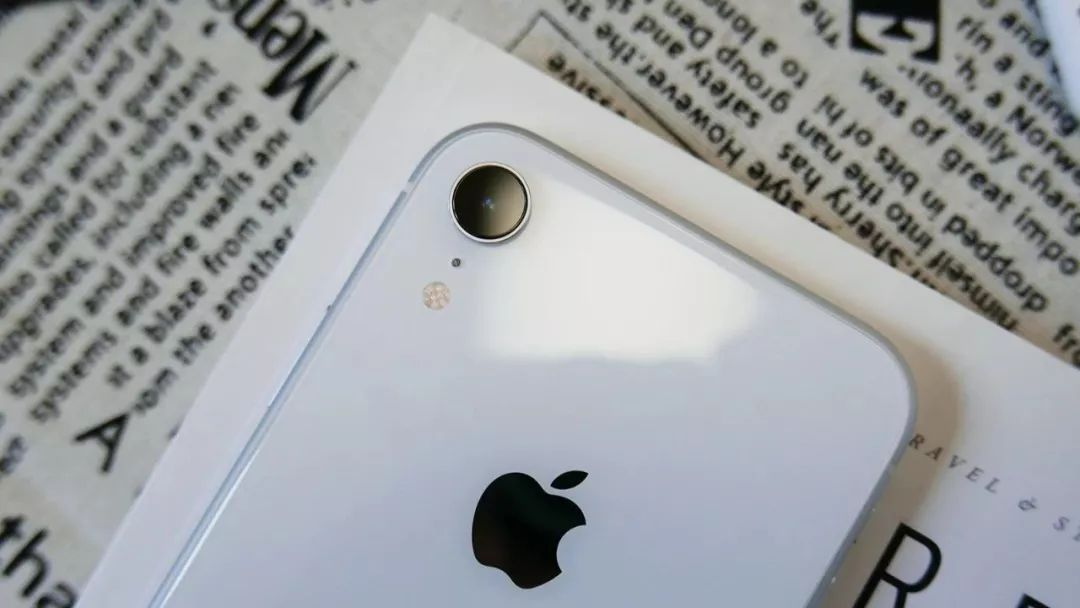
\includegraphics[width=0.7\textwidth]{iPhone-dual-micphone.jpeg} 
		\caption{iPhone8的次麦克风手机位于摄像头附近}
		\label{fig: iphone-dual-microphone}
		%\vspace{0.8cm} % 用来调整和下方文字的间距
	\end{figure}
	
	手机上设有的两个电容式麦克风尽管作用不同,但是其性能相同,对环境中声音信号的收集能力基本没有差别。如果利用双麦克风系统的时间同步(主麦和降噪麦都是集成于同一个设备的,底层数据的收集也是同步录制,故信号是完全时钟同步的)特性,即使两个麦克风(如图\ref{fig: samsung-dual-microphone})之间的距离较短(16cm左右,不同手机略有差异),也可以根据双麦采集的信号计算出声源信号到达两个麦克风的相差的采样点数,并进而计算(估计)出声源到双麦的到达时间差(TDOA),不仅如此,利用双麦克风系统智能手机也规避了两路信号时钟同步的问题。
	
	\begin{figure}[H]
		\centering
		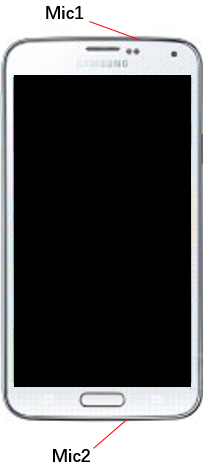
\includegraphics[width=.3\textwidth]{samsung-dual-microphone.png} 
		\caption{双麦手机,以三星S5手机为例}
		\label{fig: samsung-dual-microphone}
		%\vspace{0.8cm} % 用来调整和下方文字的间距
	\end{figure}
	
	目前国内外也已经有许多基于双麦系统实现以声源定位为基础的有趣的研究成果。例如Sun ke利用双麦克风智能手机进行手势轨迹感知\cite{VSkin};Aarab 使用双麦克风节点定位的思路测算说话人的位置\cite{DMArrays};Jian Liu使用智能手机进行键盘输入的感知\cite{snoop}。
	
	\section{智能手机的传感器}
	
	随着科技的发展,智能手机已经不只是一个通信工具,更是一个具有复杂功能的电子设备。大多数的ios和Android设备都有许多内置传感器,用来测量屏幕方向,运动和各种环境条件,这些传感器检测环境并捕获高度精度的数据信息,非常适合用来测量设备的三维移动和定位,以及实时监测周围环境,例如可以跟踪设备的重力传感器推断用户的手势和动作,同样天气应用中将会使用设备集成的湿度和温度传感器。智能手机的内置传感器可分为硬件层和软件层两种\cite{Google_Sensor}。硬件层的传感器是设备内置的物理组件,这类传感器通过直接获取特定的环境信息(如角度变化,三轴加速度,地磁场强度等)来采集数据。软件层的传感器则不是物理设备,其数据则是从一个或者多个硬件传感器中获取,例如线性加速度传感器。具体可参考表\ref{table: Android Sensor}。本章将会简述实验中涉及使用的几种传感器。
	
	\begin{table}[htbp]
		\caption{Android 平台支持的传感器类型}
		\centering
		\begin{tabular}{cccc}
			\hline 
			传感器	& 类型 & 说明 & 常见用途\\
			\hline
			\text{ACCELEROMETER} & 硬件 & 加速力 & 动态检测\\
			\text{AMBIENT\_TEMPERATURE} & 硬件 & 环境室温 & 监测气温\\
			\text{GRAVITY} & 软件或硬件 & 重力 & 动态检测 \\
			\text{GYROSCOPE} & 硬件 & 旋转速率 & 旋转检测 \\
			\text{LIGHT} & 硬件 & 环境光级(照度 & 控制屏幕亮度 \\
			\text{LINEAR\_ACCELERATION} & 软件 & 加速力 & 监测单个轴向上的加速度\\
			\text{MAGNETIC\_FIELD} & 硬件 & 环境地磁场 & 创建罗盘 \\
			\text{ORIENTATION} & 软件 & 旋转角度 & 确定设备位置 \\
			\text{PRESSURE} & 硬件 & 环境气压 & 监测气压变化 \\
			\text{PROXIMITY} & 硬件 & 物体到屏幕的距离 & 通话过程中手机的位置 \\
			\text{RELATIVE\_HUMIDITY} & 硬件 & 环境的相对湿度 & 露点,绝对湿度和相对湿度 \\
			\text{ROTATION\_VECTOR} & 软件或硬件 & 设备 & 动态检测和旋转检测\\
			\text{TEMPERATURE} & 硬件 & 设备 & 监测温度 \\
			\hline
		\end{tabular} 
		\vspace{0.2cm}
		\label{table: Android Sensor}
	\end{table}
			
		在传感器框架下采用三轴坐标系,其坐标系是相对于设备屏幕设定的,其设定如图\ref{fig: sensor}所示。对于后续介绍的的陀螺仪,加速计,以及地磁传感器,上述三轴坐标系均试用。		
		
		\begin{figure}[H]
			\centering
			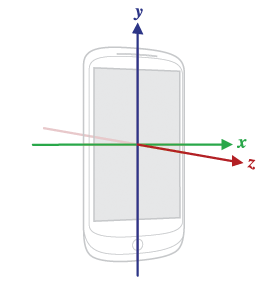
\includegraphics[width=0.4\textwidth]{sensor.png} 
			\caption{传感器坐标系}
			\label{fig: sensor}
			%\vspace{0.8cm} % 用来调整和下方文字的间距
		\end{figure}
		
			
		\subsection{陀螺仪}
		
		陀螺仪,其原理为角动量守恒定理,是一种用于感知测量和维持方向的装置。陀螺仪常用于导航,定位等系统。在Android系统中,陀螺仪测量的是围绕设备的x,y与z轴的旋转速率(弧度/秒)。通常情况下,我们利用陀螺仪的输出数据对时间进行一次积分,从而获得角度随时间变化累积的转角。但是,在本文中判定设备是否“静止”的问题上,对陀螺仪的时刻输出设定一个硬阈值,当输出数据的(绝对值)超过阈值是,即可认为在设备处于运动中。从而避免积分中的漂移问题。
			
		\subsection{加速度传感器}
		
		加速度传感器又称为加速计,用于测量设备在运动状态下的加速度的传感器。高灵敏度的加速计用于飞机和导弹的惯性导航系统中\cite{houanlu},在无人飞行器中,加速计有利于保持稳定飞行。加速计的应用相当广泛,几乎所有的智能手机都包含加速计。尽管加速计的数据中包含了重力场的成分,但是在本文的使用中并不计较其细节,因此我们不对其进行深入解析。目前的智能手机下对加速计的应用很多,例如常见的计步器\cite{jibuqi},微信“摇一摇”等。
						
		\subsection{磁力传感器}
		
		磁力传感器又称磁力仪,高斯计,是用于测量地球磁场的仪器。谈及磁力计,其主要的应用就是手机自带的指南针。在Android系统中,开发者不仅提供了获取磁力值的接口,同时也提供了磁力计与加速计结合获得方向的接口,因此,通过这方面的应用,将会给用户一个地理方位的指示。
			
		\subsection{屏幕方向传感器}
		
		方向传感器属于软件传感器,安卓平台提供方向传感器用于判断设备的位置。其数据是通过加速度传感器和磁场传感器共同获得的。至于其算法细节我们不必去关心。由于繁重的处理操作,因此方向传感器的准确度和精确度都是会降低的。具体而言,方向传感器在倾角为0时才可靠。根据官方文档的描述,Android2.2(API级别8)已经弃用屏幕方向传感器,Android4.4W(API级别20)已经弃用屏幕方向传感器类型。因此,Android系统提供了另一种方法来来获取屏幕方向值,当我们注册加速计和地磁传感器后,便可以通过调用 开发者提供的getRotationMatrix()方法和 getOrientation()方法来获取屏幕方向值。屏幕方向传感器常应用VR,AR,指南针等应用。

	
	\section{信号时延计算原理}
	
		对于具备双麦的智能手机,其主麦和降噪麦都处在“相同”的环境下,因此采集到的两路音频信号必然具有较强的相关性。当我们要求解某一个声源的空间位置时,计算出声源到达两个麦克风的信号时延往往有着重要的作用。对于到达时间差(TDOA)的获取主要有两种方法。
		
		第一种方法依赖于对信号到达时间(TOA)的测量(或计算),通过信号到达时间的差值来求得。基于到达时间的方法对系统的时间同步要求就会很高,但是在信道传输特性相似的情况下,这种办法可以减少多径效应带来的误差。以二维空间为例,如图(\ref{fig: tdoa-diagram}),根据信号到达时间可以得到关于到达时间差的方程如下:
		
		\begin{align}
			\sqrt{(x-x_1)^2+(y-y_1)^2} - \sqrt{(x-x_3)^2+(y-y_3)^2} &= c(t_1-t_3)\\
			\sqrt{(x-x_2)^2+(y-y_2)^2} - \sqrt{(x-x_3)^2+(y-y_3)^2} &= c(t_2-t_3)
		\end{align}
		
		由于依赖于TOA的值,微小的测量误差或者同步信号误差,就会引起TOA较大的误差,进而可能导致计算出的TDOA的精度降低,因此在后续的实验中没有采用这种方式求解时延。
		
		\begin{figure}[H]
			\centering
			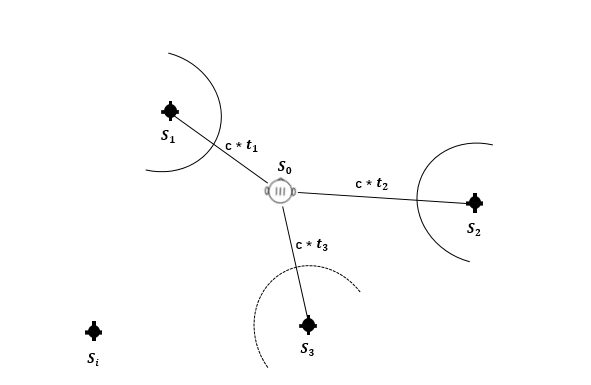
\includegraphics[width=0.7\textwidth]{tdoa_diagram.png} 
			\caption{TDOA算法示意图}
			\label{fig: tdoa-diagram}
			%\vspace{0.8cm} % 用来调整和下方文字的间距
		\end{figure}
		
		
		第二种方法是将采集到的信号进行相关运算,从而得到到达时间差(TDOA)的值。在实际应用中,系统往往很难做到严格的同步,因此在大多数的定位方案中,也常常用相关估计的方法求解TDOA的值,再进行后续的定位计算。在主流的基于无线传感网的定位方案中,这种方法对网络的要求低,故而通过该方法测量(计算)更具有实践意义。
		
		广义互相关的基本思想是对已经经过滤波等信号处理的两路信号$x_1(t)$和$x_2(t)$,求其互相关函数,其原理框架如图(\ref{fig: GCC})所示,其公式表达为:
		
		\begin{equation}
		\tau_{\text {delay }}=\underset{t \in \mathbb{R}}{\arg \max }((f \star g)(t))
		\end{equation}
		
		\begin{figure}[H]
			\centering
			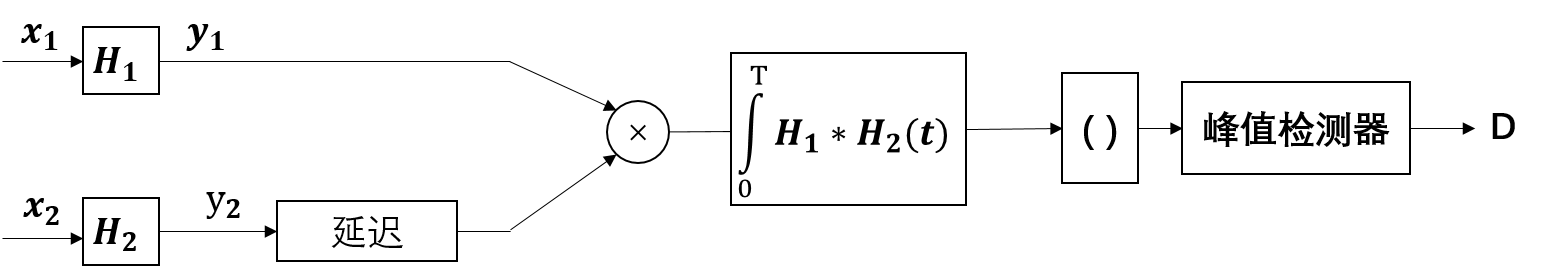
\includegraphics[width=.95\textwidth]{GCC.png} 
			\caption{互相关函数求解时延流程}
			\label{fig: GCC}
			%\vspace{0.8cm} % 用来调整和下方文字的间距
		\end{figure}	
		
		在利用线性卷积计算时,常常可以借助线性卷积的关系来实现利用频域FFT的方式计算互相关,这种方法将比传统的时域计算法极大的减少计算量。根据维纳辛钦定理:平稳信号的自相关函数与其功率谱密度互为傅里叶变换对,因此相对应的,利用频域下的功率的互功率谱可以计算时域的互相关函数。最后通过峰值检测器求解出时延。需要说明的是,麦克风采集的信号是离散的,因此时延可以看作是几个采样点数的差距,通过麦克风的采样率,我们将可以把计算的采样点数的差距转换成时间的差值。
	
	\section{基于到达时间差的定位算法设计}
	
		上一节简要描述了利用互相关估计求解信号时延的方法,这一小节将会描述利用求解出的到达时间差(TDOA)进行后续的声源定位。
		
		\subsection{二维空间下的定位分析}
		
		我们首先从二维空间下进行定位分析。首先可以明确的是,根据到达时间差,结合声速($v_{sound}$)我们可以求解出声源到两个麦克风的距离差($\Delta d$),从而由方程(\ref{2D_equation_1})因此在二维空间下,相对于手机中心和手机坐标系,我们可以得到一个以智能手机麦克风节点为焦点的双曲线,而声源则在其中的某一支曲线上。同理,当我们移动手机至别的位置,那么就又可以得到一支曲线,如图(\ref{fig: 2D_hyperbola}),则两个曲线的交点就是声源的所在位置。
		
		\begin{equation}
		\begin{aligned}
			&\sqrt{(x-{mic_1}_x)^2+(y-{mic_1}_y)^2} - \sqrt{(x-{mic_2}_x)^2+(y-{mic_2}_y)^2}\\
		  = & c \cdot \Delta t= d_1 \label{2D_equation_1}
		\end{aligned}
		\end{equation}
		
		\begin{figure}[H]
			\centering
			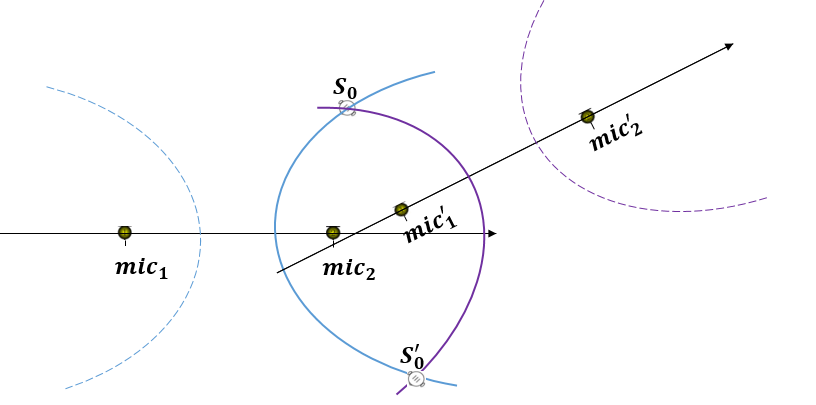
\includegraphics[width=0.8\textwidth]{2D_hyperbola.png} 
			\caption{2维双曲线定位}
			\label{fig: 2D_hyperbola}
			%\vspace{0.8cm} % 用来调整和下方文字的间距
		\end{figure}		
		
		\subsection{三维空间下的定位分析}
		
		拓展至三维空间中,同样,我们可以根据到达时间差,计算出声源到两个麦克风的距离差,因此在三维空间中,如图(\ref{fig: 3D-Hyperboloid})我们可以根据公式(\ref{3D_equation_1})得到一个双叶双曲面,而声源则可以在其中的某一个面上。同理,通过改变位置,我们可以获得更多的双曲面,进而求解出声源的所在位置。
		
		\begin{equation}
		\begin{aligned}
			&\sqrt{(x-{mic_1}_x)^2+(y-{mic_1}_y)^2+(z-{mic_1}_z)^2} - \sqrt{(x-{mic_2}_x)^2+(y-{mic_2}_y)^2+(z-{mic_2}_z)^2}\\
		  = & c \cdot \Delta t= d_1 \label{3D_equation_1}
		\end{aligned}
		\end{equation}
		
		\begin{figure}[H]
			\centering
			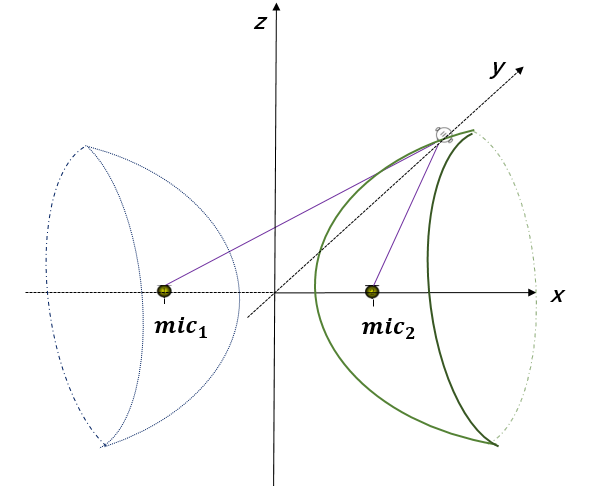
\includegraphics[width=0.7\textwidth]{3D-Hyperboloid.png} 
			\caption{3维双曲面定位}
			\label{fig: 3D-Hyperboloid}
			%\vspace{0.8cm} % 用来调整和下方文字的间距
		\end{figure}	
		
		\subsection{离线计算下的定位算法分析和设计}
		
		通过公式\ref{2D_equation_1}和公式\ref{3D_equation_1},不难看出,关于声源位置的方程组是非线性的。而且,一方面,我们不能保证到达时间差(TDOA)的测量总是不存在误差的,另一方面,我们也知道声速也并非固定不变,正如公式\ref{v_speed}所描述的那样,因此对于测量(计算)出的到达时间差,必然会存在或多或少的误差,这对后面定位精度的影响也是不可预测的。但是,由于我们变换双麦的位置,因此就可以获得很多组数据,大量数据的冗余,使得该定位问题也就转换成了非线性的最优化问题。由于二维情况可以看作三维情况下的一种特殊情况,也就是$z = {mic_i}_z$,因此只对三维空间下的情况进行分析。
		
		\begin{equation}
		   v_s = 331.3 + 0.606 * Temperature \label{v_speed}
		\end{equation}
		
		为缩小搜索空间,在麦克风位置的布置上,可以采用固定其中一个麦克风结点的方式,如图(\ref{fig: 3D-Hyperboloid2}所示,因此根据到达时间差(TDOA),可以得到如下的方程组。
		
		\begin{equation}
			 r_i^2 = (x-x_i)^2 + (y-y_i)^2 + (z-z_i)^2 \label{3D_equation_2}
		\end{equation}
		
		\begin{equation}
			r_0^2 = (x-x_0)^2 + (y-y_0)^2 + (z-z_0)^2 \label{3D_equation_3}
		\end{equation}
		
		\begin{equation}
			\Delta r_i = r_i - r_0 = c\Delta t_i, i = 1,2,3,...,m \label{3D_equation_4}
		\end{equation}
		
		式中,$r_i$为声源到不同位置下的$mic_2$的距离,$\Delta r_i$为声源到固定的$mic_1$的距离,c为声波的传播速度,$\Delta t_i$为不同位置下$mic_2$与$mic_1$的到达时间差。
		
		\begin{figure}[H]
			\centering
			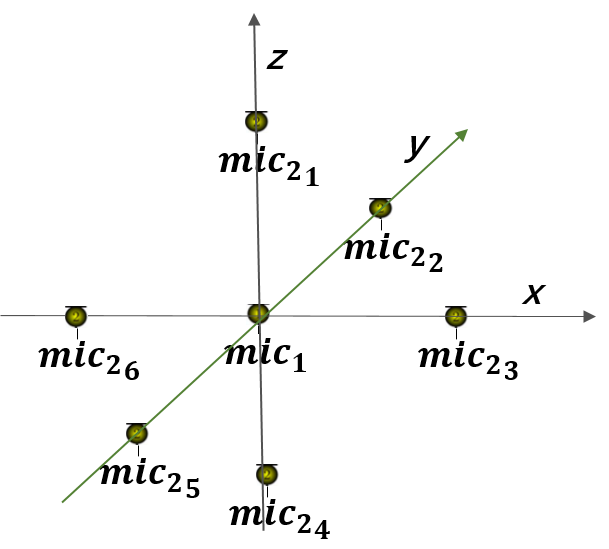
\includegraphics[width=0.7\textwidth]{3D-Hyperboloid2.png} 
			\caption{3维结点布置示意}
			\label{fig: 3D-Hyperboloid2}
			%\vspace{0.8cm} % 用来调整和下方文字的间距
		\end{figure}
		
		下面简要分析在三维空间下,基于Chan的到达时间差定位算法\cite{Chan3DTDOA}。由公式\ref{3D_equation_2}和\ref{3D_equation_3}不难得到:
		
		\begin{equation}
		\begin{aligned}
			R_{i,0}^2 & = r_i^2 - r_0^2 \\
					  &	= (x-x_i)^2 + (y-y_i)^2 + (z-z_i)^3 - (x-x_0)^2 - (y-y_0)^2 - (z-z_0)^2
		\end{aligned}
		\end{equation}
		
		\begin{equation}
		\begin{aligned}
			\Delta r_i & = r_{i,0} = r_i - r_0\\	
			  		   & = \sqrt{(x-x_i)^2 + (y-y_i)^2 + (z-z_i)^3} - \sqrt{(x-x_0)^2 + (y-y_0)^2 + (z-z_0)^2}  
		\end{aligned}
		\end{equation}
		
		\begin{equation}  
		\begin{aligned}
		& r_i^2 = K_i - 2x_ix - 2y_iy - 2z_iz + x^2 + y^2 + z^2 \label{3D_equation_5}\\
		& K_i = x_i^2 + y_i^2 + z_i^2
		\end{aligned}
		\end{equation}
		
		而由基本的定义则有:
		
		\begin{equation}  
			r_i^2 = (r_{i,0}+r_0)^2 \label{3D_equation_6}
		\end{equation}
		
		将公式\ref{3D_equation_6}代入\ref{3D_equation_5}中,于是有
		
		\begin{equation}
		\begin{aligned}
			r_{i,0}^2 + 2r_{i,0}r_0 + r_0^2 = K_i - 2x_ix - 2y_iy - 2z_iz + x^2 + y^2 + z^2 & \Longrightarrow\\
			r_{i,0}^2 + 2r_{i,0}r_0 + (x-x_0)^2 + (y-y_0)^2 + (z-z_0)^2 = K_i - 2x_ix - 2y_iy - 2z_iz + x^2 + y^2 + z^2 & \Longrightarrow\\
			r_{i,0}^2 + 2r_{i,0}r_0 = K_i - 2x_ix - 2y_iy - 2z_iz + 2x_0x + 2y_0y + 2z_0z - (x_0^2 + y_0^2 + z_0^2) = r_i^2 - r_0^2 & \Longrightarrow\\
			r_{i,0}^2 + 2r_{i,0}r_0 = -2(X_{i,0}\cdot x + Y_{i,0}\cdot y + Z{i,0}\cdot z) + K_i - K_0 & \Longrightarrow\\
			X_{i,0} = x_i - x_0,  Y_{i,0} = y_i - y_0,  Z_{i,0} = z_i - z_0 & \Longrightarrow
		\end{aligned}
		\end{equation}
		
		将上式转换为矩阵形式
		
		\begin{equation}
			R_{i,0}^2 = r_i^2 - r_0^2 = -2{
			\left[ 
			\begin{array}{c c c}
				X_{i,0} & Y_{i,0} i & Z_{1,0}
			\end{array} 
			\right ]}{
			\left[ 
			\begin{array}{c}
				x\\
				y\\
				z
			\end{array}
			\right ]} + K_i - K_0
		\end{equation}
		
		通过上面所描述的这种转化,可以消除未知数的平方项,而只保留了一次项,根据i的不同取值,可以得到了一系列的线性方程组。
		
		\begin{equation}
		\begin{aligned}
			& \frac{1}{2} * {
				\left[ 
					\begin{array}{c}
						R_{1,0}^2 - K_1 + K_0 \\
						R_{2,0}^2 - K_2 + K_0 \\
						...
					\end{array} 
				\right ]}
				= -{
				\left[ 
					\begin{array}{ccc}
						X_{1,0} & Y_{1,0} & Z_{1,0} \\
						X_{2,0} & Y_{2,0} & Z_{2,0} \\
						  ...   &  ...    &   ...
					\end{array}
				\right ]}*{
				\left[ 
					\begin{array}{c}
						x\\
						y\\
						z
					\end{array}
				\right ]} & \\
			& h = \frac{1}{2} * {
				\left[ 
				\begin{array}{c}
				R_{1,0}^2 - K_1 + K_0 \\
				R_{2,0}^2 - K_2 + K_0 \\
				...
				\end{array} 
				\right ]}, 
			G = -{
				\left[ 
				\begin{array}{ccc}
				X_{1,0} & Y_{1,0} & Z_{1,0} \\
				X_{2,0} & Y_{2,0} & Z_{2,0} \\
				...   &  ...    &   ...
				\end{array}
				\right ]},
			h = Gz^0
		\end{aligned}
		\end{equation}

		其中$z^0$即为要求解的值。当然,由于误差的存在,所以$Gz^0\neq h$,误差向量为$\phi = h - Gz^0$。只需要3个TDOA测量(计算)值,就可以通过计算得到声源的位置(x,y,z)。但是可以通过利于冗余数据,从而可以获得更好的拟合值。于是通过加权最小二乘法获得初始的估计解,再利用估计解和其他条件进行第二次加权平均,对得到的估计值进行优化。在Chan算法定位问题\cite{Chan3DTDOA}中有具体算法的描述和分析,这一方面不是本文的重点,因此不做赘述。
		
		\subsection{在线指引下的寻迹方式}
		
		在前一小节中,我们简要描述了离线处理中,通过基于Chan的到达时间差算法计算出未知声源的方法。这种方法尽管操作方式复杂,但是却可以获得较为准确的结果。然而,在实际的定位中,在短距离的室内环境中,我们也不是对周围的事物“视而不见”,因此往往一个简单的方向指引就具有很好的参考意义。因此,对于三维的空间定位,在一定程度下,仅仅二维的指引就可以作为较好的参考方向。
		
		如图(\ref{fig: 2D_guide})中,我们获取了一个以麦克风为焦点的双曲线,同样,我们也就获得双曲线的渐进方向。而当声源距离麦克风中心较远时,渐进线的方向就是对声源方位的一个很好的指引。如果我们希望定位方式从离线状态下计算位置,转移到在线的指引我们去寻找的话,这种方向指引无疑是一种很好的途径。后文中,我们将对这个问题做具体描述。
		
		\begin{figure}[H]
			\centering
			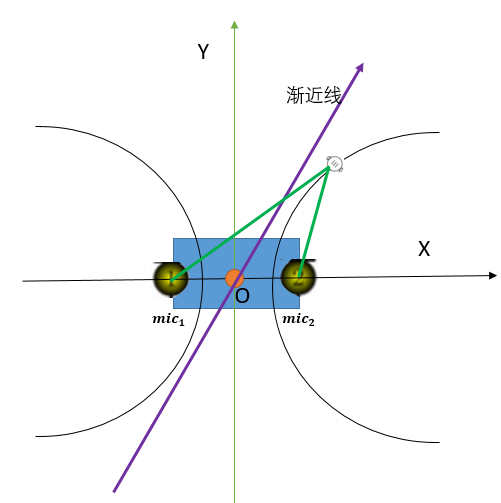
\includegraphics[width=0.7\textwidth]{2D_guide.png} 
			\caption{2维空间指引}
			\label{fig: 2D_guide}
			%\vspace{0.8cm} % 用来调整和下方文字的间距
		\end{figure}
	
%%%%%%%%%%%%%%%%%%%%%%%%%%%%%%%%%%%%%%%%%%%%%%%%%%%%%%%%%%%%%%%%%%%%%%%%%%%%%%%
\chapter{基于双麦系统智能手机的声源定位方案}\label{chapter_work}
	
	近些年来,智能设备尤其是智能手机已经普及,智能设备上传感器的集成和发展,也使得智能手机的功螚越来越丰富。在前面我们已经简述到现阶段的智能手机,都已经普及使用双麦系统,其中的降噪麦克风也是为了有效抑制我们在日常通话中的环境噪声,并且也分析到两个麦克风是时钟同步的。因此,利用智能手机的优势,通过获取同一个手机两个麦克风的声音数据,我们从中过滤出我们想要的声音信号,就可以得到两路严格同步的声音信号,并进而可以通过广义互相关的方法求解出声源到两个麦克风的信号时延,对计算出的信号时延进行后续的处理,就可以实现一些有意义的功能\cite{zhouxin}。
	

	本章首先对室内定位系统构建中的挑战做一些描述,随后阐述系统的构建方案,最后,在前一章的基础上,详细描述数据收集方案,采集到的底层信号的预处理过程,并分析其特征。因为声音信号的非平稳性,所以预处理操作尤为重要。本章节将会描述利用双麦克风手机实现定位功能的诸多细节性工作,从而用于后续的定位分析。
	
	\section{室内定位方案中的挑战}
		
		前文中我们谈及了许多利用声波进行室内定位的方案,以及利用双麦手机进行手势识别等的系统,因此,利用双麦智能手机进行室内定位的想法也就有了实践的意义。然而在系统构建中,依然存在着诸多挑战。
		
		\subsection{单个智能设备感知}
		
			使用单个智能手机去实现定位局限就在于主流设备仅仅只是做到双麦立体音录制,前文中我们说明到根据双麦的位置和时延可以获得一个位置下的双曲面方程(二维则为双曲线),显然,通过一个双曲面自然是无法求解出声源的位置的,理论上,可以根据多个双曲面相交是可以求解出交点位置,从而计算出声源的位置的,但是这显然是需要至少三个麦克风同时录制的。而且,双麦手机的麦克风之间的距离也是固定不变的,因此信号时延的计算结果也是有局限的。补充说明的是,经过调研,例如iphone 5s,Samsung Galaxy Note 3等设备具有三麦系统,但是采用这些设备进行研究,一方面成本高昂,另一方面开发者也没有提供处理三个麦克风数据的接口,因此实现难度也会更大。
			
		\subsection{惯性测量单元的精度误差}
		
			在假定声源静止的情况下去计算声源的三维位置,需要多个双曲面的构建,因此需要对双麦的空间位置进行改变(这里我们只考虑双麦智能手机)。然而,这也依赖于双麦中心位置的变化的测量是较为精确的。如图\ref{fig: IMU},一方面涉及加速计求解中心移动量,一方面涉及陀螺仪求解三轴旋转量,两者的累积误差都会大大影响到定位的精度。

			\begin{figure}[H]
				\centering
				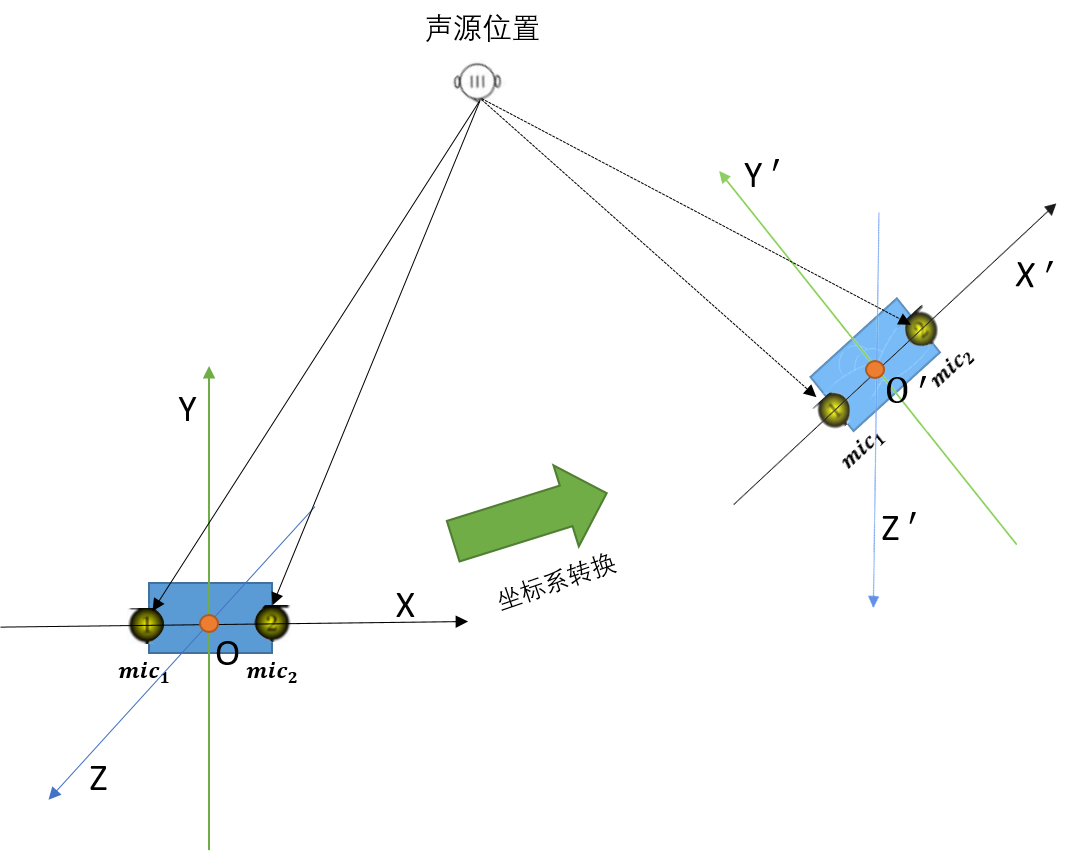
\includegraphics[width=.9\textwidth]{IMU.png} 
				\caption{坐标系转换}
				\label{fig: IMU}
				%\vspace{0.8cm} % 用来调整和下方文字的间距
			\end{figure}
		
	\section{系统构建思路}
	
		本文提出了针对定位的两种策略,分别是离线计算策略和在线指引策略。
		
		第一种离线计算方案,如图(\ref{fig: strategy1})是根据多位置录制数据,通过数据冗余的优点拟合出声源位置。通过多次部署双麦手机,对智能设备进行复用,同时以先验知识的方式获取双麦结点的位置,从而避免使用惯性测量单元带来的累积误差。
		
		\begin{figure}[H]
			\centering
			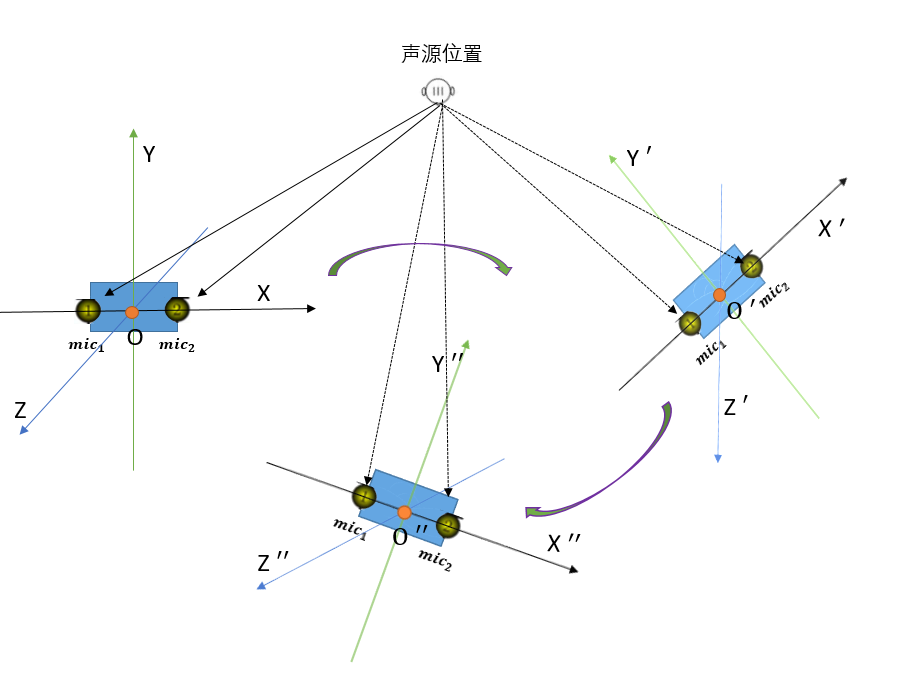
\includegraphics[width=.8\textwidth]{strategy1.png} 
			\caption{离线计算模型}
			\label{fig: strategy1}
			%\vspace{0.8cm} % 用来调整和下方文字的间距
		\end{figure}
		
		第二种在线指引方案,如图(\ref{fig: strategy2})由于单个双曲面(双曲线)无法实现定位,但是仍然可以通过具有指引功能的渐近方向来让我们在行走的过程中不断靠近声源,从而实现一种在线的定位方案。尽管对声源位置并不是一次性求解,但是基于过程的探测依然会指引我们靠近声源。由于并非“视而不见”,方向指引至足够靠近时,我们便可以找到声源。
		
		\begin{figure}[H]
			\centering
			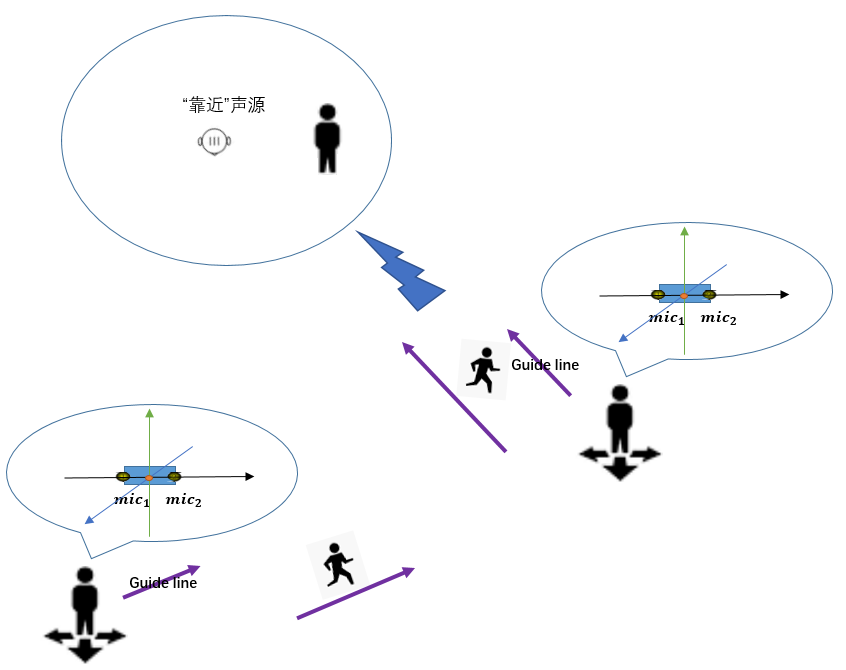
\includegraphics[width=.8\textwidth]{strategy2.png} 
			\caption{在线指引模型}
			\label{fig: strategy2}
			%\vspace{0.8cm} % 用来调整和下方文字的间距
		\end{figure}
		
	
	\section{离线数据预处理流程}
	
		本小节中,首先介绍离线状态下的数据预处理流程,并逐渐过渡到系统后续使用的在线指引模型的数据处理流程。由于麦克风收集的信号是一种非平稳的带宽信号,因此需要对收集的信号进行预处理操作,否则,由于噪声等环境因素的影响,会使得实验效果很不理想。
		
		在离线数据处理流程中,通过智能手机收集声音文件并记录为一个wav文件,通过MATLAB分析该wav文件,最终计算出到达时间差。该离线数据算法处理流程是为了通过处理一段时间窗口内,设备没有发生大幅度状态变化(包括角度,位置等参数)的情况下,计算出静态声源相对于该位置的方向(Speaker Direction Finding (SDF))。在分析阶段,包括滤波,加权移除异常点,加窗分帧,端点检测等必要操作,在一段时间窗口内的处理流程具体如下图所示(\ref{fig: offline-flowchart}).
		
		\begin{figure}[H]
			\centering
			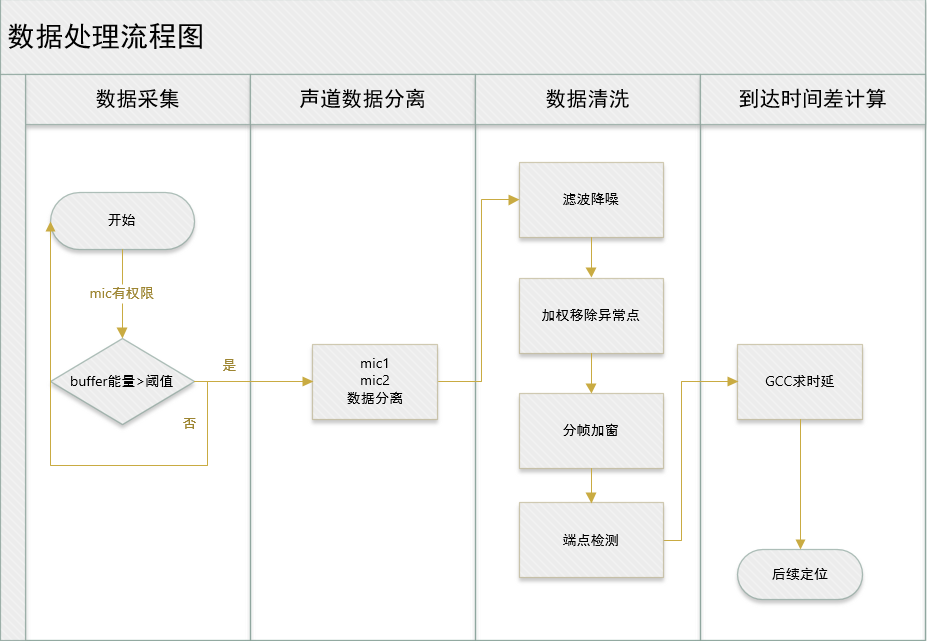
\includegraphics[scale = 0.5]{offline-flowchart.png} 
			\caption{离线数据处理流程}
			\label{fig: offline-flowchart}
			%\vspace{0.8cm} % 用来调整和下方文字的间距
		\end{figure}
	
	\section{数据采集}
	
		本文利用一部具有双麦系统的智能手机(Samsung Galaxy S5)作为信号采集的设备,在分析阶段,使用MATLAB科学工具对采集到的声音信号进行处理和显示。我们利用另一台智能手机(Vivo Y93S)发出了一个频率在2000Hz-2700Hz变换的线性调频信号,如图\ref{fig: dual-microphone-data}所示,图中蓝色的标记为LY的数据以及红色的标记为RY的数据,分别代指两个麦克风采集的数据。图中的上一部分图中,横坐标代指数据采样点,纵坐标是对数据进行标准化后的结果,因此无量纲。但是在下部分图中,横坐标是标准化的频率,单位为$\pi * $radians/sample(频率标准化的相关概念不做赘述,可以参考\cite{Normalized_frequency}),纵坐标为能量谱,这里我们很容易看出两个麦克风的采集的数据的能量谱是非常接近的,换句话说,两个麦克风的采集能力非常接近。这里我们对原始数据取样其中发声部分中连续的400个样本点。如图\ref{fig: dual-microphone-data1}所示,同样我们依然可以看出两个麦克风的采集能力是非常接近的,另一方面,即便我们暂时无法确定到达时间差(TDOA)的值,但是我们可以清晰看出收集到两路声音数据只是差了几个样本点的,因此只要计算出信号相差的样本点数,就可以根据采样率(44.1kHz)进而求解出TDOA的近似的结果。
		
		\begin{figure}[H]
			\centering
			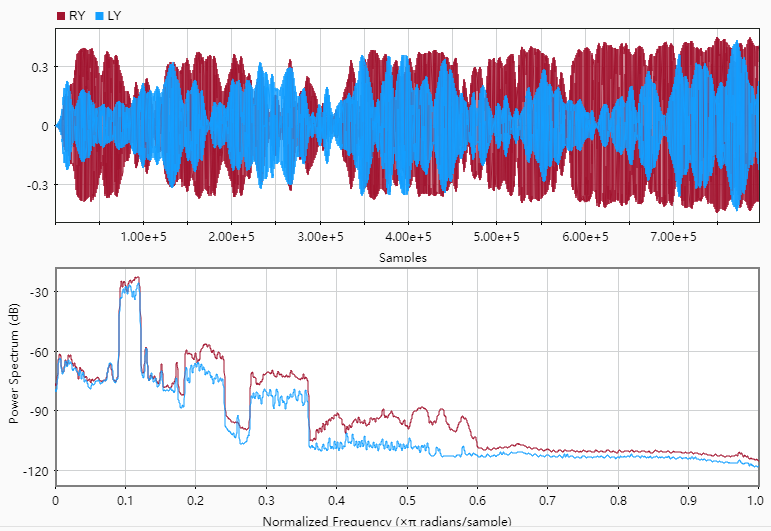
\includegraphics[width=\textwidth]{dual-microphone-data.png} 
			\caption{双麦克风信号}
			\label{fig: dual-microphone-data}
			%\vspace{0.8cm} % 用来调整和下方文字的间距
		\end{figure}
	
		\begin{figure}[H]
			\centering
			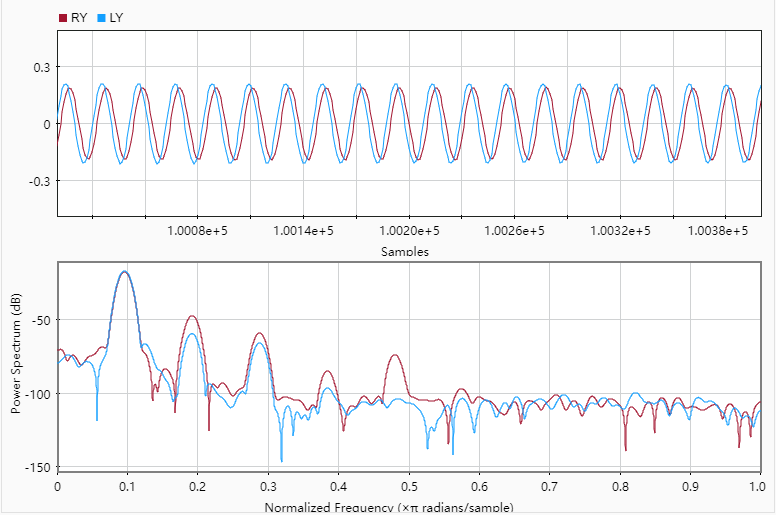
\includegraphics[width=\textwidth]{dual-microphone-data1.png} 
			\caption{双麦克风信号取样}
			\label{fig: dual-microphone-data1}
			%\vspace{0.8cm} % 用来调整和下方文字的间距
		\end{figure}
		
		下表中\ref{table: parameters-of-S5}展示了测试手机(Samsung Galaxy S5)的参数,后续实验中使用了华为mate20手机作为实验设备,S5和华为手机上也都配备了两麦系统,目前智能手机录音的采样频率主要为44.1kHz,16bit量化。大部分手机都支持包括8kHz/8bit、11.025kHz/8bit、22.05kHz/16bit和44.1kHz/16bit,因此两个设备并无太大差异。
		
		\begin{table}[H]
			\setlength{\belowcaptionskip}{7pt}
			\caption{SamSung Galaxy S5测试设备参数}
			\centering
			\begin{tabular}{ccc}
				\hline 
				参数 & 描述 \\
				\hline
				麦克风距离 & 16cm \\
				最高采样频率 & 44.1kHz\\
				方向传感器 & 不支持\\
				\hline
			\end{tabular} 
			\vspace{0.2cm}
			\label{table: parameters-of-S5}
		\end{table}
	
		但是需要补充说明的是,智能手机在录制性能上还是有些许差异的,通过调研,华为手机(\ref{fig: huawei})在录制方面从频谱低端到大约17kHz都能出色的再现自然的声音,而三星手机则在高频端有更好的性能。由于设备的局限性,在后续声源方面,依然可以通过非超声波作为信号载体实现定位。另一方面,华为手机的空间感方面性能也更优,对数据采集的灵敏度也高一些。所以在后续实验中以华为手机作为接收设备,而用普通的Vivo手机发出声波即可。
		
		\begin{figure}[H]
			\centering
			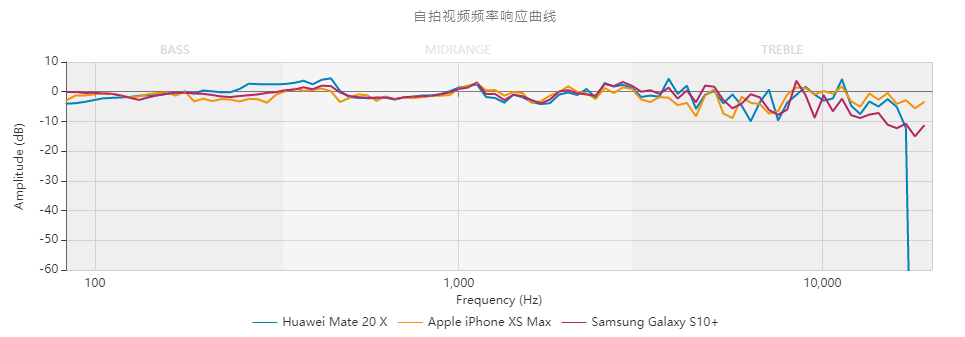
\includegraphics[width = \textwidth]{huawei.png} 
			\caption{华为手机录制性能}
			\label{fig: huawei}
			%\vspace{0.8cm} % 用来调整和下方文字的间距
		\end{figure}
	
		本文采用具有双麦系统的S5手实时采集环境的声音信号,在Android系统底层获取的声音数据实际是个一维数组,当然利用MATLAB进行读取,会转换成两个一维数组,分别代表两个麦克风的数据。在原始的底层存储中,一维数组的值即是采集到的数据。如图\ref{fig: sound-data}所示,实验中,我们采用16bit的stero的格式进行采集,因此根据图中的存储方式很容易分别获得两个麦克风的数据,并且两组数据是完全满足时钟同步的。为了区分声源和环境噪声,本文中对采集的信号设置了一个能量阈值,当每个buffer中信号的能量超过于该阈值时,则认为采集到的了声源数据,而当buffe中的信号能量低于该阈值时,则没有采集到的声音数据。最后对采集到的数据进行后续的信号处理。
		
		\begin{figure}[H]
			\centering
			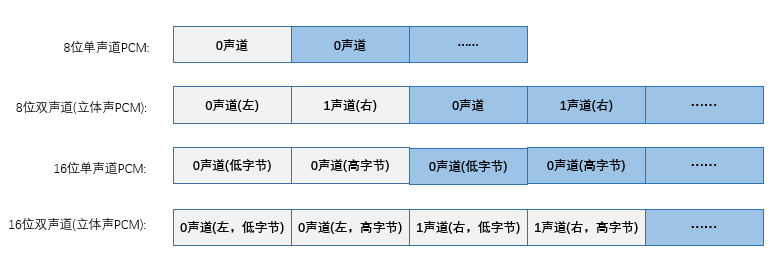
\includegraphics[width = \textwidth]{sound-data.png} 
			\caption{数据存储方式}
			\label{fig: sound-data}
			%\vspace{0.8cm} % 用来调整和下方文字的间距
		\end{figure}
	
	\section{声音数据处理}
	
		智能手机从底层获得的两路麦克风数据中,既包括了采集到的声源信号,尽管室内环境较为安静,但是同时也会有环境噪声以及其他各种异常信号,本小节将会利用自带的滤波器除噪以降低噪声的影响,同时使用加窗移动的方式降低数据中的异常值的影响,从而实现对原始录制的信号进行清洗处理,后续将会进行分窗加帧,端点检测等为后续到达时间差的计算做准备。

		\subsection{滤波除噪}
			
			由于信号采集中也会含有噪声成分,这对我们声源定位无疑会造成很大的影响,因此我们应该去除非声源发声的成分,提高声源的成分。常见的去噪方式就是使用滤波器,这里我们使用带通滤波器,降低环境中噪声的干扰。在MATLAB通过filter,designfilter函数我们很容易实现我们需要的功能,在后续的在线算法处理流程中,因为程序运行在Java平台上,所以Android系统方面可以通过使用dsp-collection这一个jar包来满足我们需要的功能。
			
			例如当我们的声源频率范围在2000Hz-2700Hz时,那么在除噪的过程中,我们就需要通过一个带通滤波器,减益非该频率范围的成分。在滤波器阶数方面,对于室内环境噪声,采用6阶滤波器已经可以满足需求。如图(\ref{fig: data-unfiltered},\ref{fig: data-filtered})所示,横纵坐标信息同图(\ref{fig: dual-microphone-data})。通过滤波器的数据滤波,频率不在指定频率范围的音频信号,将会被大大减益,从而降低了环境噪声对后续信号时延的精度影响。
			
			
			\begin{figure}[H]
				\centering
				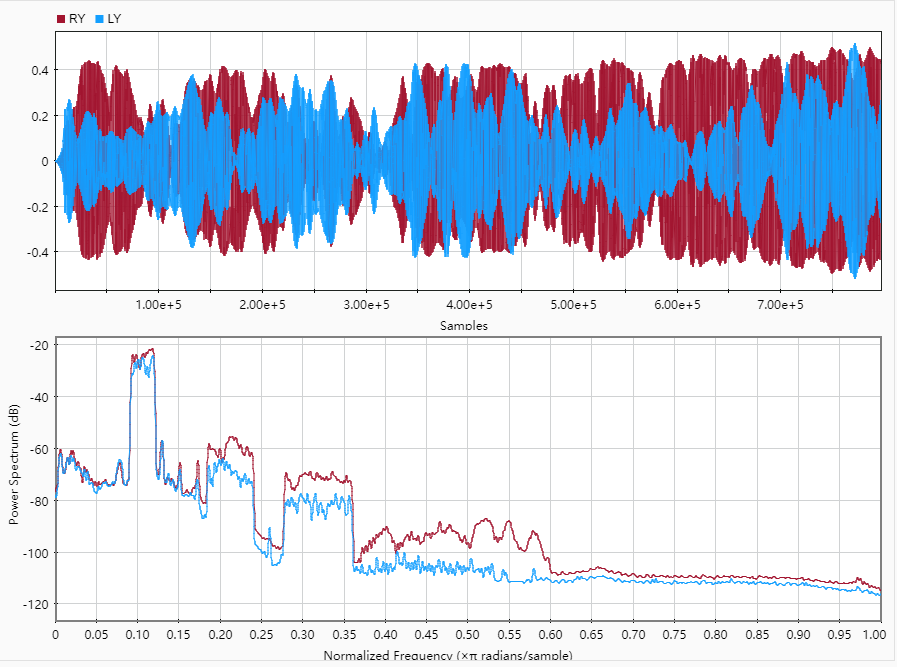
\includegraphics[width=\textwidth]{data-unfiltered.png}
				\caption{信号除噪之前}
				\label{fig: data-unfiltered}
				%\vspace{0.8cm} % 用来调整和下方文字的间距
			\end{figure}
		
			\begin{figure}[H]
				\centering
				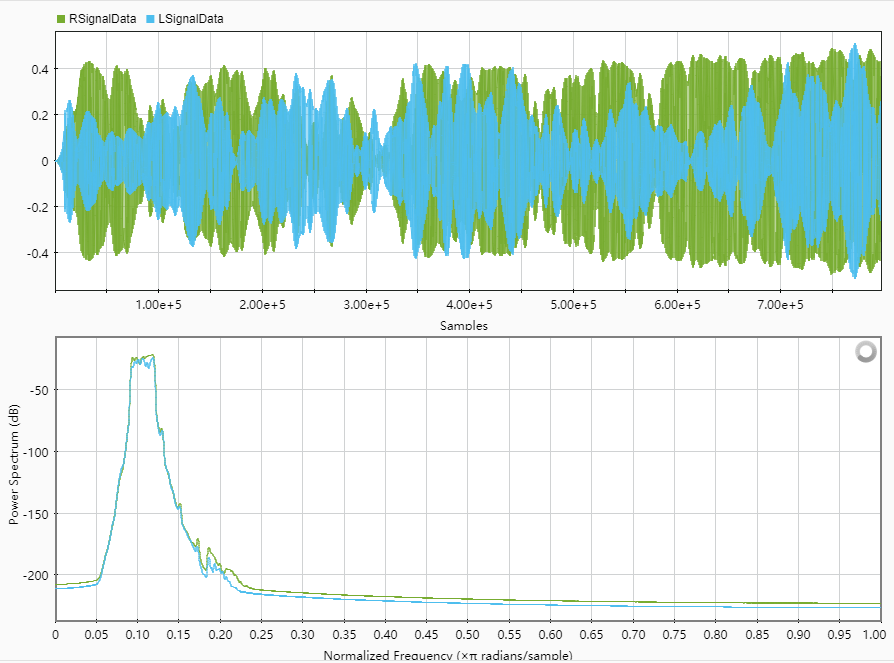
\includegraphics[width=\textwidth]{data-filtered.png}
				\caption{信号除噪以后}
				\label{fig: data-filtered}
				%\vspace{0.8cm} % 用来调整和下方文字的间距
			\end{figure}
					
		\subsection{异常点移除}
		
			对实验结果影响较大的还有异常数据,例如在看似稳定的声音信号中,由于降噪麦和主麦底层下硬件的问题,仍会有一些突变的声音信号。这里采用对两路声音信号分开进行处理。值得一提的是,由于采样率高达44.1kHz,所以处理过程中去掉一些数据并不会造成较大的影响。这里,我们采用滑动窗口的方式,使用加权平均移动(\text{WMA}\cite{Moving_average})的方式进行处理。加权平均移动认为:同一个窗口内的不同的数据对目标值都有着不相同的权重因子,因此目标值就可以看成窗口内数据和一个固定的权重函数的卷积。由于数据本身异常点并不是很多,并且使用传统的\text{WMA}就可以获得较好的效果,因此记$\text{signal}_t$为t时刻的数据,采用下面的公式更新t时刻的信号值:
			
			\begin{equation}
			\begin{aligned}
				\text{signal}_{t_{new}} = \text{WMA}_{t}&=\frac{n p_{t}+(n-1) p_{t-1}+\cdots+2 p_{(t-n+2)}+p_{(t-n+1)}}{n+(n-1)+\cdots+2+1}\\
											  &=\frac{n \times \text { signal }_{t-1}+(n-1) \times \text {signal}_{t-1}+\cdots+1 \times \text {signal}_{t-n+1}}{n+(n-1)+\cdots+2+1}								 
			\end{aligned}
			\end{equation}
			
			经过上述处理后,数据变得更加光滑,并且从图\ref{fig: data-outliers-removed}中已经可以隐约可见到达时间差(TDOA)的大致范围。这里,\text{LSD}为第一个麦克风降噪后是数据,\text{LSignaData}代表降噪后数据经过异常点去除操作后的数据,声源主频率数据并不会因此受到影响。
			
			\begin{figure}[H]
				\centering
				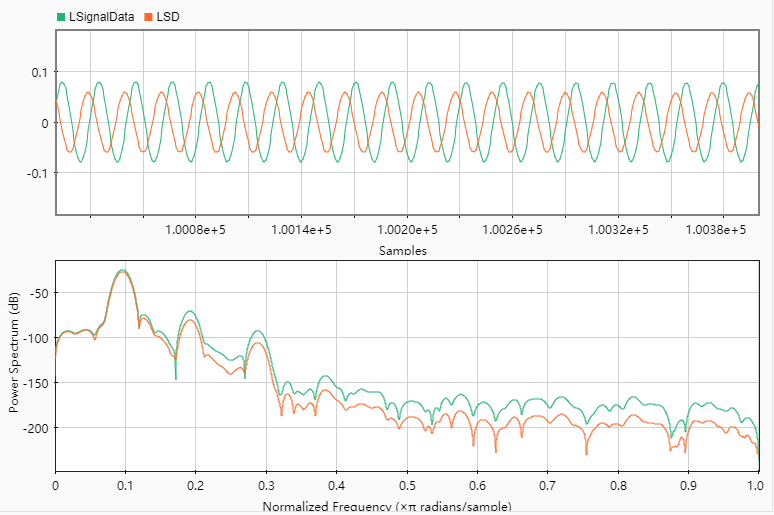
\includegraphics[width=0.9\textwidth]{data-outliers-removed.png} 
				\caption{异常点移除后的数据}
				\label{fig: data-outliers-removed}
				%\vspace{0.8cm} % 用来调整和下方文字的间距
			\end{figure}
		
		\subsection{分窗加帧}
		
			尽管我们采集到的声音信号并不是平稳的,但是在较小的时间窗口中,比如几十毫秒级别的时间测度范围下,声音信号依然是近似平稳的。基于这个想法,可以把采集的声音数据,看作是一帧一帧的小时间窗口范围的信号的组成,每一帧的信号都可以看成独立的声音信号。在这个思想下,实际就是在声音数据添加了一个滑动窗口,窗口的移动速度在窗口长度的三分之一左右即可。如图(\ref{fig: framing})所示:
					
			\begin{figure}[H]
				\centering
				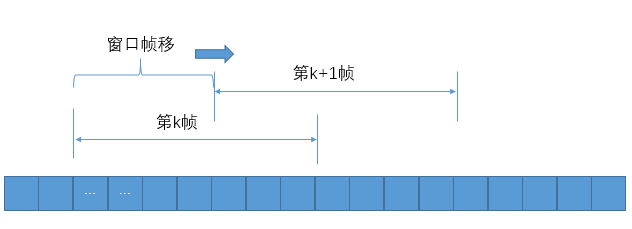
\includegraphics[width=0.8\textwidth]{framing.png} 
				\caption{数据分帧}
				\label{fig: framing}
				%\vspace{0.8cm} % 用来调整和下方文字的间距
			\end{figure}
		
			由于在信号分帧中,我们基本上是不可能做到对信号的周期性截断,常常的解决方法是在时域上对信号进行加窗以调制信号,减少信号的频谱泄露。常见的窗函数有矩形窗,汉明窗,汉宁窗,此外还有三角窗,高斯窗\cite{Window_function}。如果以N表示帧长,那么前三种窗函数的时域表达式如下所示。
			
			(1)矩形窗的时域表达式:
			
			\begin{equation}
				w(n)=\left\{
				\begin{aligned}
					&1, 0\leq n \leq N - 1\\
					&0, n = else
				\end{aligned}
				\right.
			\end{equation}
			
			
			(2)汉宁窗和汉明窗的时域表达式:
			\begin{equation}
				w(n)=a_0-(1-a_0)\cdot cos(\frac{2\pi n}{N}), 0 \leq n \leq N
			\end{equation}
			
			当$a_0$=0.5时,为汉宁窗,当$a_0=0.54(\frac{25}{46})$时,为汉明窗.
			
			对窗函数的性能区别我们不做过多描述,在制定频段的声音下,为了保持平滑,汉明窗的性能更优,但是由于声源信号是周期有规律的,因此两种窗函数在实际使用中性能接近。
			
			
		\subsection{端点检测}
		
			尽管我们采集的声音是“连续”采集的,但是仍然有可能部分数据帧中,并不没有录制到声源的信号,例如智能手机开启麦克风时,底层仍有一个异常的信号电平,这方面的超过了本文的论述内容,因此不做躲过解释。但是,即便如此,依然可以在数据处理中通过端点检测查找到有效的声源发源部分。在前文数据采集中,我们对数据采集设定了一个基于能量的硬阈值,虽然短时能量可能出现噪声特征值较大,或者声音混淆的情况,但是在实际实验中,由于室内环境噪声较小,利用短时能量依然可以满足我们的需要。对这方面的优化依可以通过参考文献\cite{Endpoint_detection}中的对数能量特征进行优化。
		
		\subsection{到达时间差计算}
			
			本小节基于前期的信号处理后,获取到两个同步的,并且噪声,异常点数据都得到有效处理的分帧加窗后的数据,随后调用第二章讲解到的GCC算法对两路信号进行到达时间差(TDOA)计算(估计)。具体原理已在前文说明,因此这里我们不再赘述其原理。
			
			由于接收到的声音信号来自于同一个声源,因此两路信号之间具有较强的相关性而与噪声无关。通过描述的广义互相关方法,我们可以得到两路信号之间的时延差。前文中我们也有说明,这里计算出的“时延”实际是两个信号相差的采样点数,但是,由于采样率为设定好的44.1kHz,因此可以通过计算出相差的采样点数,经过转换从而可以得到对应的时延,也就是实际的到达时间差(TDOA),后面我们用相差的采样点数代指到达时间差(TDOA),转换公式无需赘述。可以明确的是,以$mic_2$为标准,当TDOA < 0时,$mic_1$先接收到信号,TDOA > 0 时,$mic_1$后接收到信号,TDOA = 0 时,声波同时到达$mic_1$和$mic_2$。降至二维空间下,详情如图(\ref{fig: tdoa})所示。需要注意的是,TDOA的正负也是相对而言的,例如$mic_1$早于$mic_2$接收到信号,也就对应了$mic_2$晚于$mic_1$接收到信号。
			
			\begin{figure}[H]
				\centering
				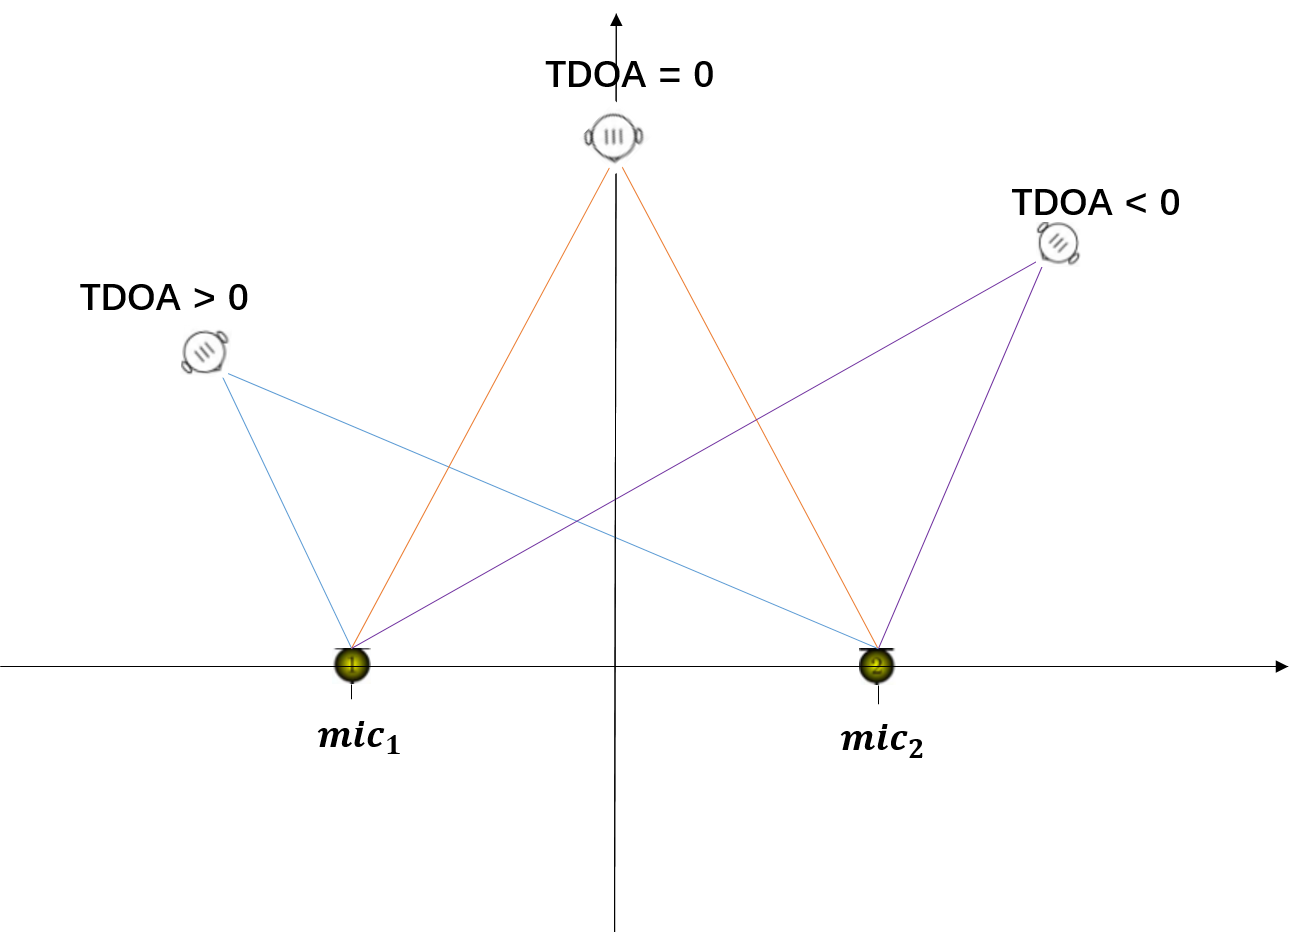
\includegraphics[width=0.8\textwidth]{tdoa.png} 
				\caption{{\text{TDOA > 0, TDOA < 0, TDOA = 0}}}
				\label{fig: tdoa}
				%\vspace{0.8cm} % 用来调整和下方文字的间距
			\end{figure}
		
		\subsection{到达时间差处理}
		
		利用双麦手机作为接收设备,计算声波到达手机双麦的时间差,高达44.1kHz的采样使得我们可以得到大量的声音数据,并且计算出很多个数据段的到达时间差。因此鉴于数据量多的优势,那么我们就可以利用此优势进行数据的筛选。即便我们的某些到达时间差测量并不是足够“精确”,但是依然可以辅助进行方向探测。
		
		回到最初的系统设置,我们设置的采样率44.1kHz,编码为16bit,我们暂时不考虑高编码编码的精确度,但显然的是,由于使用的bit数较大,因此数据量化的范围也更大,因此数据也是更精确的。对于44.1kHz的采样率,麦克风每手机一秒钟,就可以采样到44.1kHz的采样点。实验中发现,如果将太多量的数据一次性进行计算,由于声源功率较小,信号衰减等,大部分测量结果都是不准确的。然而,另一方面,即便数据过多造成了结果不够准确,但是对数据分段,对该一秒钟的部分数据进行到达时间差的计算,在原理上也是对整段数据的到达时间差的估计,因为延迟是“全局”的延迟,通过实验我们也发现了这一个问题。因此,鉴于这种思想,前文中我们也说明了对信号进行分帧加窗,当然,由于在后续实验中设备会一直处理数据,我们对每k个连续数据进行分帧。从而,对两个麦克风相同次序的数据帧进行到达时间差(TDOA)计算,依然可以得到全局的到达时间差(TDOA),如图(\ref{fig: data-split})。
		
		\begin{figure}[H]
			\centering
			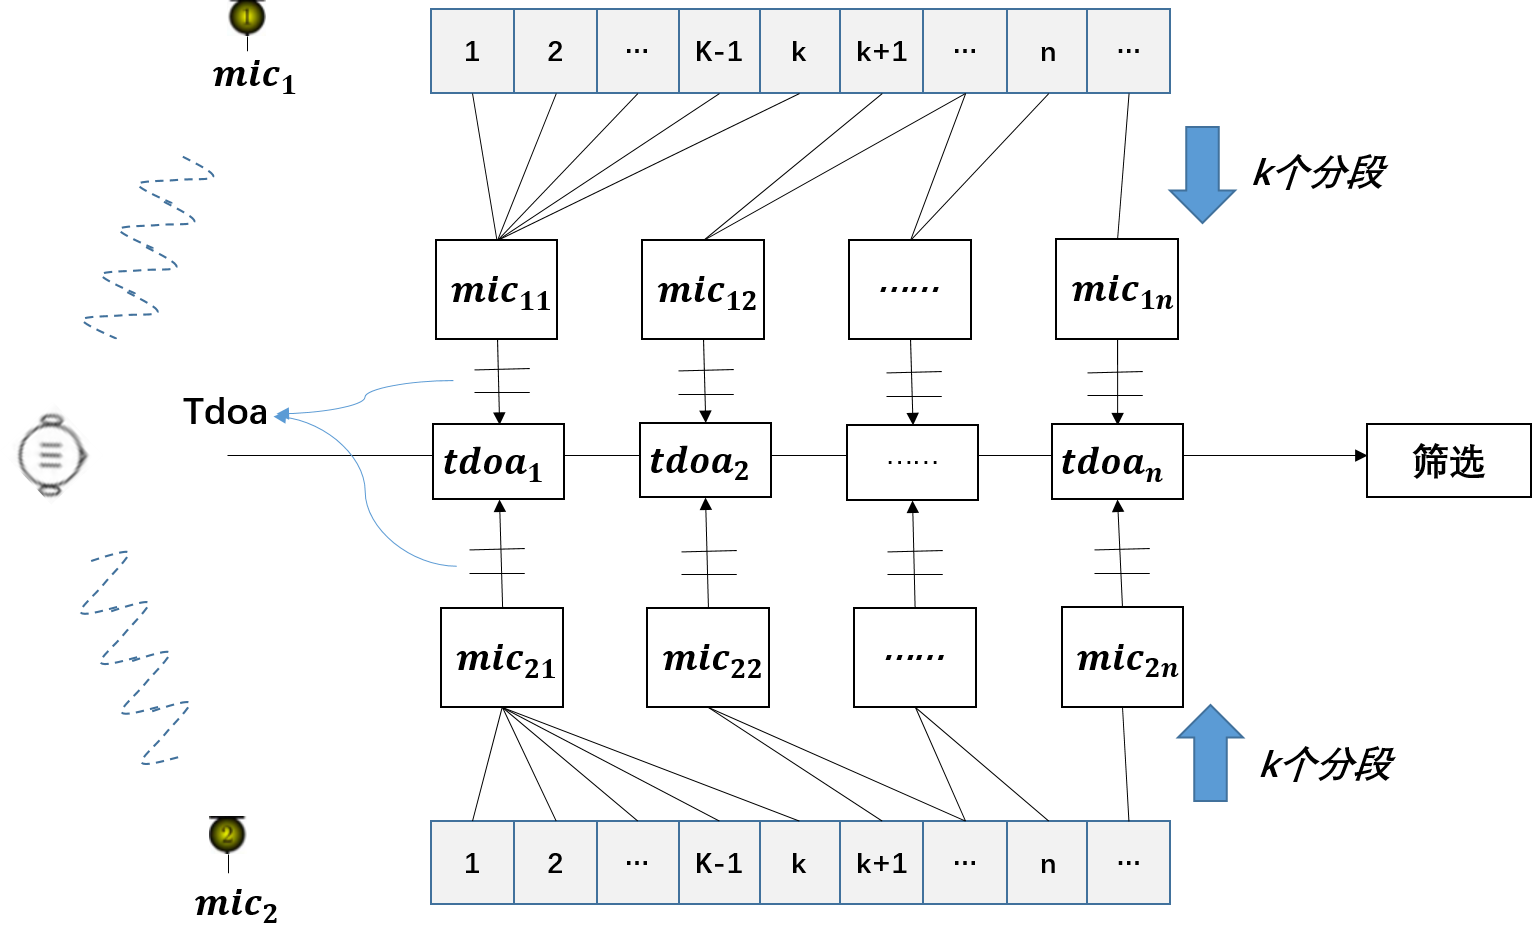
\includegraphics[width=\textwidth]{data-split.png} 
			\caption{{数据分段示意}}
			\label{fig: data-split}
			%\vspace{0.8cm} % 用来调整和下方文字的间距
		\end{figure}
		
		数据分帧之后,并进行对应的数据段的到达时间差(TDOA)的计算,从而可以产生一系列的到达时间差(TDOA)值。在实际计算中,我们设定帧长k = 2048,很明显的是,对k的设定是一个trade-off的问题,若k值太小,数据点太少,基本无法得到合理的到达时间差(TDOA)值,如果k值较大,精度会有影响,实验中k暂取用2048。由于1s中可以采集到44100个数据,因此帧移改为帧长,从而减少计算量。另一方面需要明确的时,实验中设备的麦克风距离约为16cm,因此,从采样点的角度看,到达时间差(TDOA)绝对值的最大值$|\text{TDOA}|_{\text{max}}$应该满足下式(以20℃的环境为例):
		
		\begin{align}
			|\text{TDOA}|_{\text{max}} & = 16 / v * 44100 \leq 16 / ((331.3 + 20 * 0.606) * 100) * 44100  \\
									   & = 16 / (34342) * 44100\\
									   & \approx 20.546 < 21
		\end{align}
		
		由于采样点误差必然会有0.5个采样点的误差范围,所以TDOA的范围应该在-21至21之间,这就是到达时间差采样点角度的合理值的区间。另一方面,虽然由于离散采样的问题,到达时间差(TDOA)的值最后应该取整数,但是我们也可以肯定的是,即便有0.5个采样点的误差,$\Delta distance = 0.5 / 44100 * v \leq 0.5 / 44100 * 34342 \approx 0.389cm$,对于16cm的麦克风距离来说,这个值微不足道。
		
		前面中我们提及到,每一帧的信号计算出的到达时间差应该符合或者接近于全局的到达时间差,基于这种原因,我们使用以下的数据筛选方案进行数据综合数理(下以TDOA代指采样点角度的到达时间差):
		
		(1)每m 秒中,准确来说,应该是每$\lfloor 44100 * m / 2048 \rfloor * 2048 $个数据,进行一个到达时间差的计算,在这一次的计算中,按照前文叙述的方法,每k(k=2048)个数据计算一次TDOA的计算,因此可以产生个$\lfloor 44100 * m / 2048 \rfloor$个TDOA的值。
		
		(2)对于这些计算出的TDOA的值,如果有超过一半的值相同并且介于前面所说的合理值区间,那么我们就可以认定计算的TDOA有效,并且其符号包括数值都可以用于后续的处理算法中。
		
		(3)如果无法满足(2)的条件,但是大部分值甚至所有值都是大于0或者小于0,或者等于0,只有极少的符号与整体不一致,这里我们定义极少为占比不超过1/7,那么仍然可以认为该组TDOA有效,不过此时我们只使用TDOA的符号,也就是大部分值的符号,用于后续的方位判断。对于特殊情况,我们考察这些数值的众数,如果只有一个众数,如果众数在“大部分值”占比超过一半,那么我们使用该众数作为TDOA的数值;如果存在多个众数,并且数值差值不超过2,并且所有众数在“大部分值”中的占比超过一半,我们可以使用这些众数的均值作为TDOA的数值使用,否则,在(3)中,我们只使用TDOA的符号。
		
		(4)如果(2)(3)的处理条件都无法满足的话,则认为这一次计算的结果无效。
		
		但是,当TDOA不为0的时候,信号能量会有较为明显的对比,因此对于符号的判断基本都可以保证,因此大部分测量结果至少可以返回一个合理的TDOA符号,因此大致方向可以确定。并且在离线处理中,取m=1,就可以满足我们的实验需求。
		
	\section{离线处理下的定位方法}
		
		图(\ref{fig: tdoa})中,如果我们以$\text{mic}_1$为左,以$\text{mic}_2$为右,根据到达时间差的符号(0,-1,1)实际可以确定对于声源与中心关系,这里我们只简单定义为左,前,右三个方向。后续说明方位的时候,我们所指方向就是这里说明的左,前,后。
	
		由到达时间差(TDOA)我们很容易确定一个双曲线方程,对于双曲线的渐近线方向,就是对声源的很好一个指示,至少在2D的范围中是很好的一个标准。这里我们根据到达时间差(TDOA)的值和麦克风距离,就可以计算出渐近线的角度(方向),前文中我们对此进行了较为详细的描述。后续说明角度的时候,我们所指角度就是这里说明的角度。
		
		在室内环境(图\ref{fig: indoor})下,我们需要在整个空间坐标系下确定每次设备的所处的位置,也就是说,已经确定了图\ref{fig: indoor}中$\text{Position}_i$的位置,随后我们在每个位置下录取一段音频,并进行到达时间差的计算,由于设备在三维空间中可以有很多的位置,因此,我们可以得到一系列的$\text{Position}_i$,以及对应的$X_i,Y_i,Z_i,TDOA_i$。我们利用已经比较成熟的前文所描述的Chan算法即可计算出后续的结果,然而在实际操作中,由于位置精度测量本身的误差,因此可以尽可能的固定其中一个麦克风的位置,既方便与计算,同时其误差也小于变换位置后的测量误差。
		
		\begin{figure}[H]
			\centering
			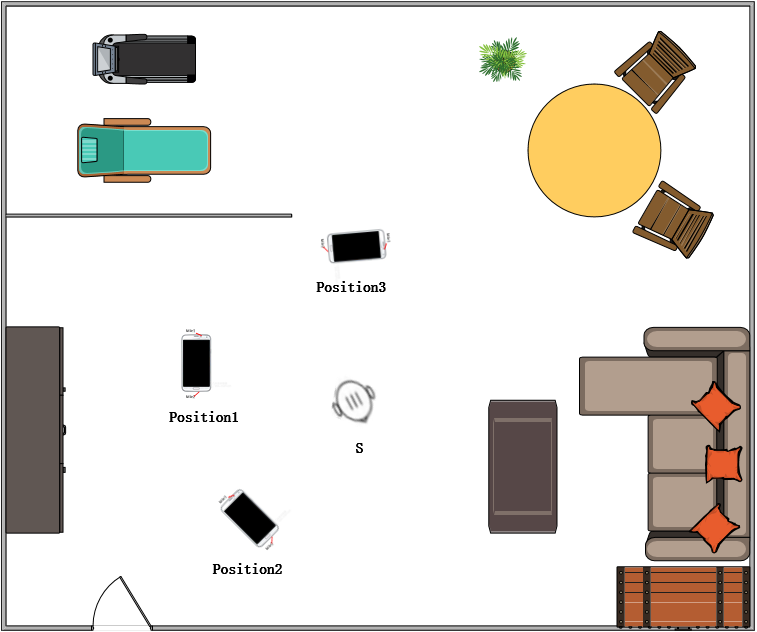
\includegraphics[width=0.9\textwidth]{indoor.png} 
			\caption{{室内环境}}
			\label{fig: indoor}
			%\vspace{0.8cm} % 用来调整和下方文字的间距
		\end{figure}
		
	
	\section{离线计算到在线指引的迁移}
		
		前面已经描述离线计算的定位犯法,正如第二章描述的那样,适当的方向指引依然有很强的指示作用。这一节讲解在线指引模型,通过降低对精度的要求,实现在线平台下的指引方案。
	
		\subsection{概念阐述}
			
			对数据的离线处理和定位计算尽管可以获得更为精确的结果,但是在实际操作中过于复杂,并且在实际寻找的过程中,我们也并不是“视而不见”,简单的提示信息或许就可以帮助我们的进行探测,因此我们降低了实际需求,从精确到3D指引降至2.5D的探测范围。因此在离线定位算法的处理的基础上,我们提出了数据在线的处理流程。
		
			这里我们需要更新之前的处理流程,因为在数据在线处理流程中,麦克风处于持续的录音状态,因此有效声音提取部分也就不是那么重要,在前面的讲解中,我们指出无效声音段并不是声音信号的主体,因此可以直接抛弃一些数据。尽管数据的在线处理流程也可以看作多个离线处理的组成,但是在实际操作中,我们还是不希望在寻找过程中,在一个位置上长期停留,后续,我们引入一些机制进行一些状态的判断。
			
			首先,我们需要提出一种降维的思想。如图\ref{fig: 3D-dimension-reduction},记智能手机屏幕所在平面为$\text{P}_1$,声源实际位置$\text{S}$与两个麦克风$\text{mic}_1$,$\text{mic}_2$所在平面为$\text{P}_2$,记$\text{P}_1$和$\text{P}_2$构成二面角为$\alpha$,在$\text{P}_2$中,声源位置$\text{S}$与智能手机中心的连线$\text{l}_1$与麦克风所在直线$\text{l}_2$夹角为$\beta$,声源在平面$\text{P}_1$的投影$\text{S}^{'}$与智能手机中心的连线$\text{l}_3$与麦克风所在直线$\text{l}_2$夹角为$\gamma$.显然很容易得到$\tan \gamma = \cos \alpha \cdot \tan \beta$.图中$\text{l}_4$为平面$\text{P}_1$上与麦克风所在直线$\text{l}_2$夹角为$\beta$的直线。尽管$\alpha$的值我们无法获知,但是计算出一个粗略的$\beta$,依然有一定的指导意义,因为在平面$\text{P}_1$上,声源投影的位置$\text{S}^{'}$的方向角$\gamma = \arctan (\cos \alpha \cdot \tan \beta)$。
			
			\begin{figure}[H]
				\centering
				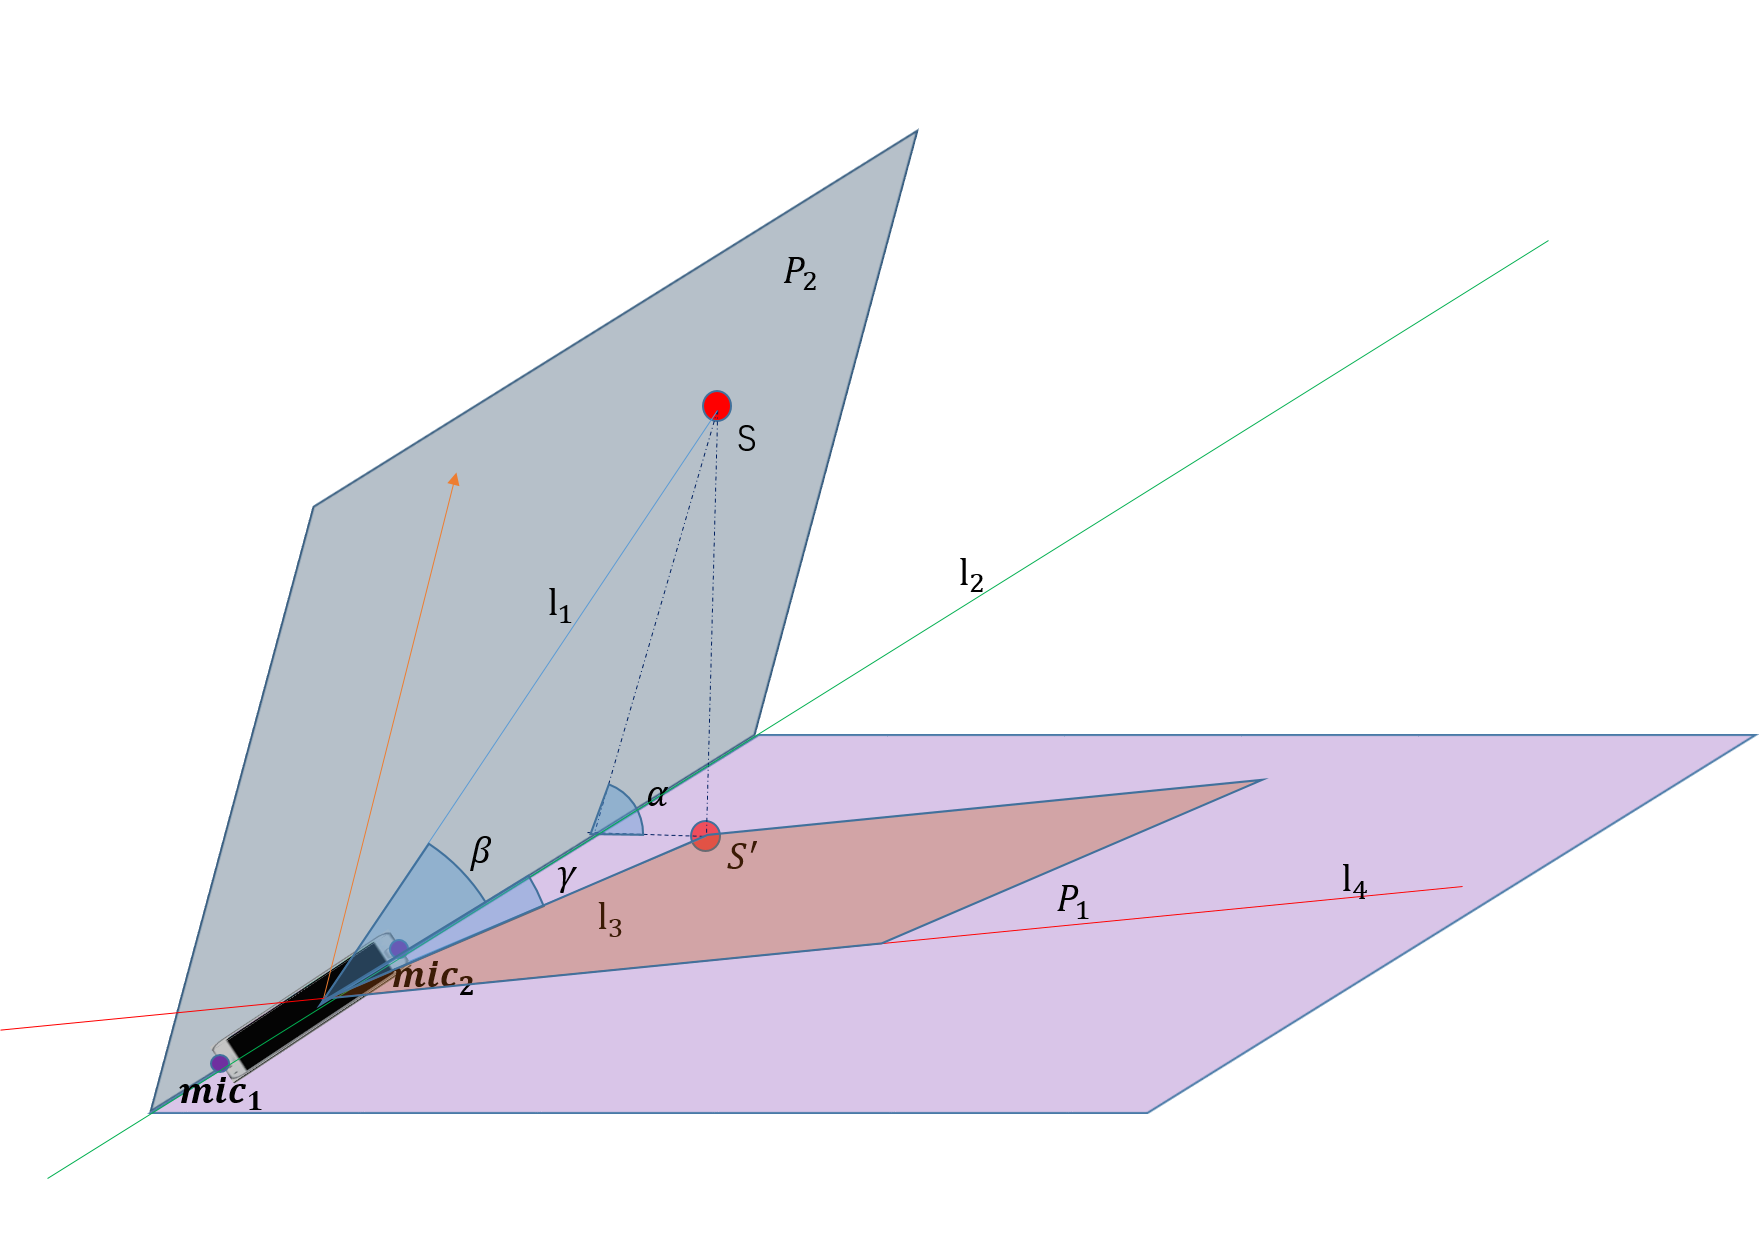
\includegraphics[width=0.65\textwidth]{3D-dimension-reduction.png} 
				\caption{{3D降维指引}}
				\label{fig: 3D-dimension-reduction}
				%\vspace{0.8cm} % 用来调整和下方文字的间距
			\end{figure}
			
			如果在平面$\text{P}_1$上仍使用$\beta$作为指引的方向,那么,这里就会产生一个角度上偏离误差$\Delta \theta = \beta - \arctan (\cos \alpha \cdot \tan \beta)$,显然当$\alpha$越大时,误差$\Delta \theta$越大(这里$\alpha$不超过90度)。显然在实际运行过程中,我们并不需要考虑这种情况。这是因为实际过程中,智能手机并非是固定不动的,因此,稍微的转动就可以使得二面角发生较大的变化。如图\ref{fig: 3D-dimension-reduction2}所示,当手机位于$\text{Loc}_1$时,二面角$\alpha$达到90度,但是只要稍微转动至$\text{Loc}_2$处,就可以获得一个新的$\alpha$,甚至我们可以把手机移动到$\text{Loc}_3$处。当手机的转动已经不能造成二面角$\alpha$较大的变化时,我们也就来到了声源投影位置的附近区域,这样,声源的位置我们也就大致获得了。
			
			\begin{figure}[H]
				\centering
				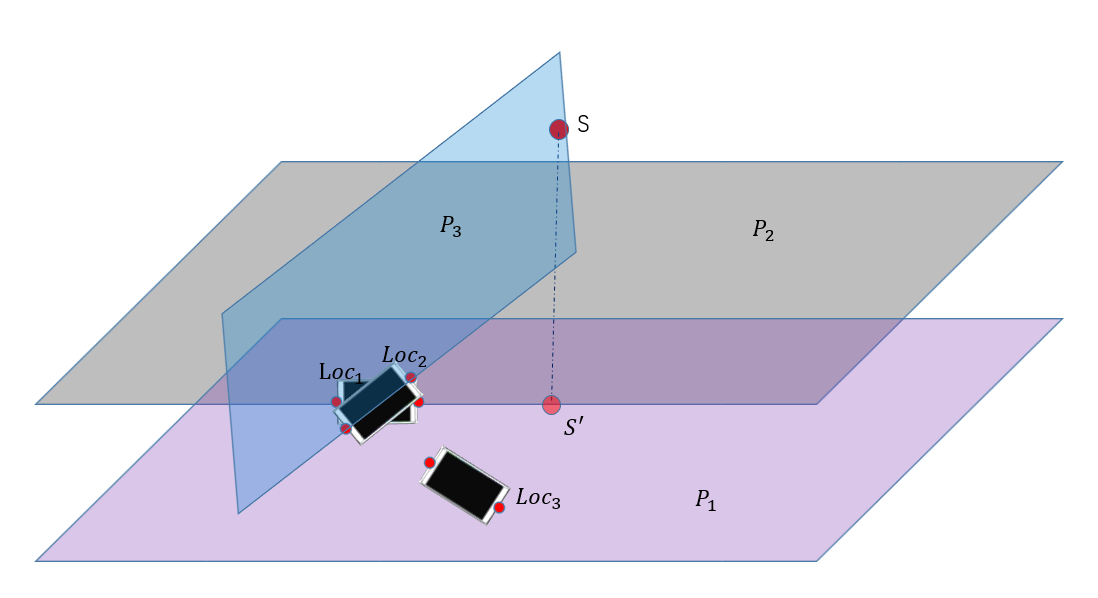
\includegraphics[width=0.8\textwidth]{3D-dimension-reduction2.png} 
				\caption{{手机状态改变}}
				\label{fig: 3D-dimension-reduction2}
				%\vspace{0.8cm} % 用来调整和下方文字的间距
			\end{figure}	
		
		\subsection{在线处理算法模型}
			
			在在线指引算法的模型下,我们需要引入一些机制,因为在在线指引的模型下,我们需要一个低要求的方向指引,而不再是准确的三维坐标。而且,在寻迹中,智能手机是动态移动的,而我们在计算到达时间差的过程中,必然是要保证麦克风位置时不变的。因此对于状态的判断就显得尤为重要。其次为了能够给予较好的方向指引,我们混合了地理方向等判断。
			
			前文中我们提到了麦克风采样率为44.1kHz,因此在到达时间差和方向计算下,我们依然用滑动窗口的方式,窗口长度为5s,而窗口移动的速度则设置为1s,因此,第从5s开始后,系统将会每一秒反馈一个计算出的结果进行指引。
			
		\subsection{状态判别}
		
			在手机状态判别问题上,主要包括静止状态判定,声源位置方位判定。
			
			一方面,在静止状态判定问题上,我们自然可以采用时域下某个指标积分后的结果进行衡量,但是由于Android自带的传感器必然存在温差,零漂的问题,因此,我们采用陀螺仪瞬时值进行衡量。
			
			另一方面,在声源位置方位判断上,只是为了粗略估计声源是否发生了位置移动。在前文中,我们提及了声源相当于手机中心的“左右”位置关系,因此在在线指引的模型下,我们通过对“左右”关系进行检测,如图(\ref{fig: state-change})所示,当我们等待过程中,如果系统反馈的声源方向在“左”($T_0^{'}$)“右”($T_0$)关系上不恒定,那么我们将认为声源的位置在改变。尽管在后续实验中并不会出现这种情况,但是这是对实际应用下系统性能的优化。
			
			\begin{figure}[H]
				\centering
				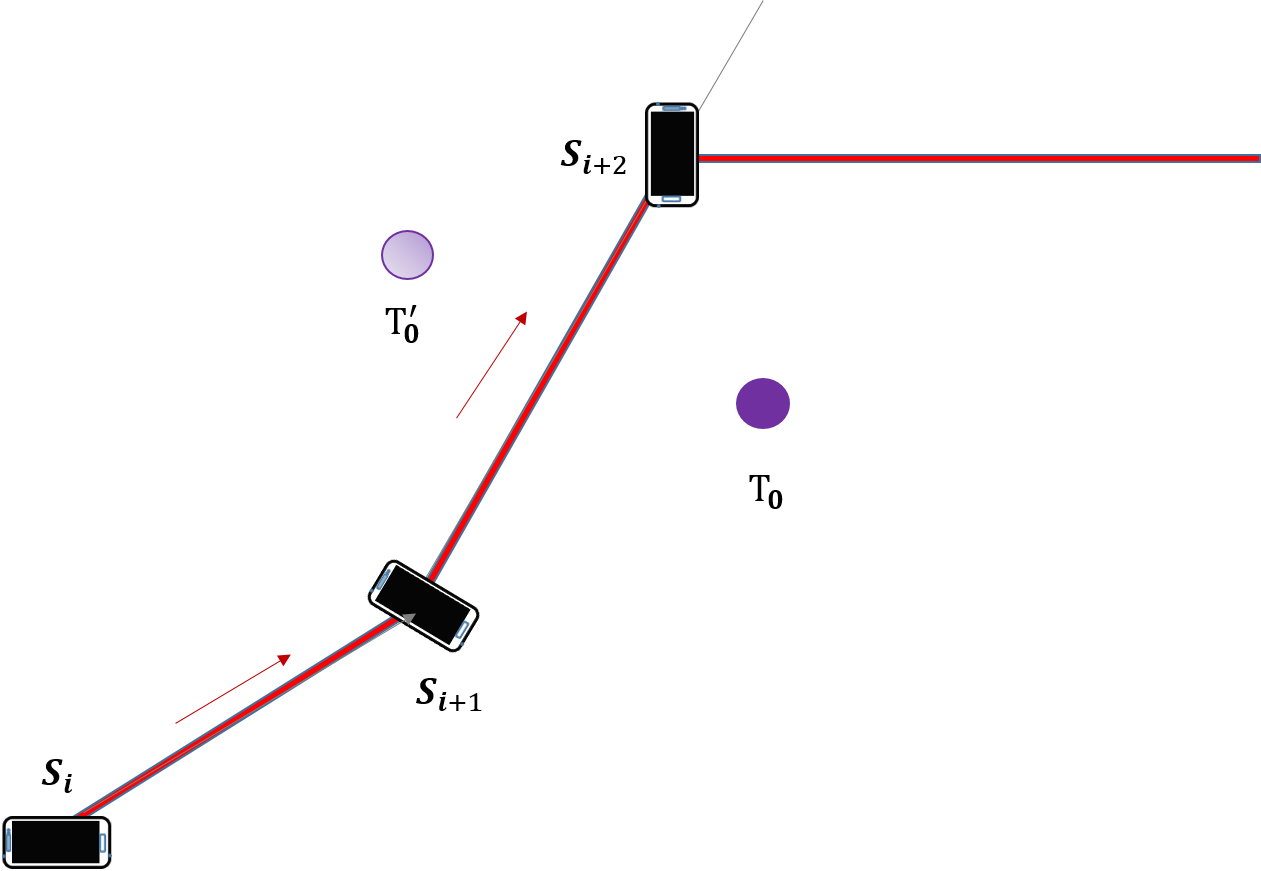
\includegraphics[width=0.7\textwidth]{state_change.png} 
				\caption{{状态判别}}
				\label{fig: state-change}
				%\vspace{0.8cm} % 用来调整和下方文字的间距
			\end{figure}	
						
		\subsection{陀螺仪数据使用}	
		
			首先我们需要确定手机处于“静止”状态,这里,尽管可以围绕麦克风所在直线旋转,但是在在线指引的模型下,我们不需要有这种操作,因此我们把这种状态也当作“非静止”的状态进行处理。以下给出一组围绕X轴依次旋转90,180,270,360度的采集到的数据,如图(\ref{fig: gyro}),分别表示三轴采集到的陀螺仪数据,横坐标为采样点,纵坐标陀螺仪采集数值,数据的单位为弧度/秒。从中可以看出,在设备绕x轴旋转的过程中,y,z两轴同样会有数据的波动,但是,即便存在数据的波动,依然维持在0的附近,而发生运动的过程时,陀螺仪的数据就会有很大的波动,因此为了实际的应用场景,我们对三轴设定一个硬阈值,当陀螺仪数据(的绝对值)超过阈值时,则判定为设备发生了运动。
		
			\begin{figure}[H]
				\centering
				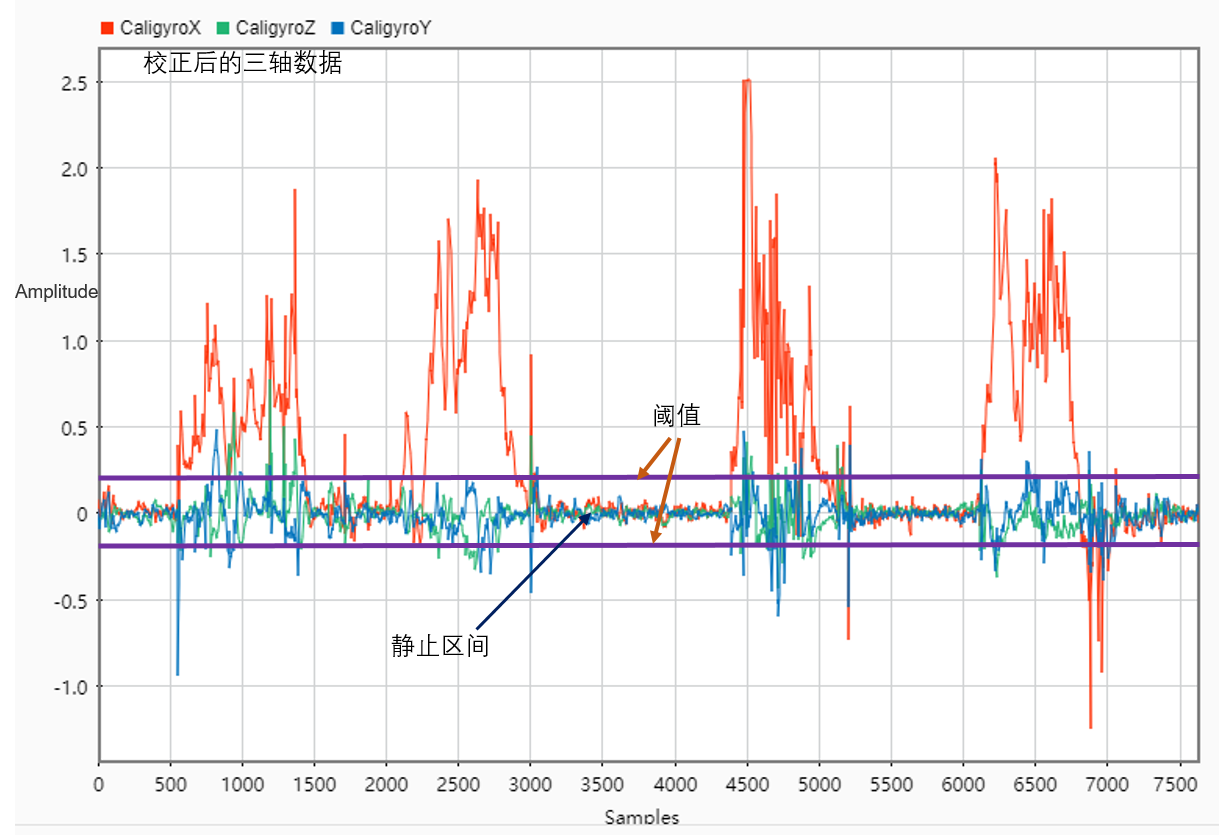
\includegraphics[width=\textwidth]{gyrohandled.png} 
				\caption{{陀螺仪三轴数据}}
				\label{fig: gyro}
				%\vspace{0.8cm} % 用来调整和下方文字的间距
			\end{figure}
		
		\subsection{加速计和磁力计的使用}	
			
			随后,为了辅助与实际方向结合,因此借用Android的加速计和磁力计,其实现细节不做过多描述。当我们在Android设备下注册了加速计和磁力计两个传感器后,就可以通过对SensorManager调用getRotationMatrix以及getOrientation,即可获得屏幕朝向与磁极的夹角,从而获取当前的方向,因此在过程中,并没有对加速计和磁力计数据的直接使用。
			
	
\chapter{模型系统实现与实验分析}
	
	本系统是对前文所述的基于双麦克风手机的声源定位方案的实现,系统包括在线指引功能,离线计算等。离线计算的呈现方式是采取手机录音和matlab计算相结合的方式,在线指引的方式是制作成一个Android系统下的智能手机应用。此外,在声源方面,也是使用了一个自制的Android系统下的智能手机应用,该应用可以发出指定的声波,用于区分声源。
	
	
	\section{开发环境与平台}
		
		\begin{enumerate}
			\item[1.] 硬件条件:
				\begin{enumerate}
					\item[1.1.] 声源设备使用的是:Vivo Y93s
					\item[1.2.] 录音设备使用的是:华为Mate20
				\end{enumerate}
			\item[2.] 系统平台:
				\begin{enumerate}
					\item[2.1.] 录音软件,声源发生软件都运行在Android系统下,
					\item[2.2.] 离线计算相关程序运行在Windows环境中,以Maltab程序的方式呈现	
				\end{enumerate}
			\item[3.] 开发工具:
				\begin{enumerate}
					\item[3.1.] 手机应用开发平台
						\begin{enumerate}
							\item[3.1.1.] Android Studio,版本号:2.3.3
							\item[3.1.2.] JRE: 1.8.0\_112
							\item[3.1.3.] JVM: OpenJDK 64-Bit Server VM by JetBrains s.r.o		
						\end{enumerate}			
					\item[3.2.] Matlab版本:9.4.0.813654 (R2018a)
				\end{enumerate}	
		\end{enumerate}
	
	\section{系统设计}
	
		在系统实现上有两种版本,正如前文描述的那样,一个版本是通过在指定位置下进行录音并保存音频为wav文件,然后通过将录音位置和波形文件导入的matlab中进行线下的计算,以定位声源的位置;另一个版本则是在手机屏幕上实时进行录音和方向反馈,通过不断的方向指引帮助我们去寻找声源。由于第一种版本除了录音阶段在智能手机上运行,其他阶段在都在matlab上运行,而且两种版本实现方式有一定的重合部分,因此会在一起进行介绍,尤以第二个版本为重。
		
		\subsection{多模块功能设计}
		
			在系统运行中,各个模块功能的并行运行是突出的。因此对在线指引系统中,系统涵盖的模块可以分为:传感器数据监听模块,录音模块,数据处理模块,显示模块等。
			
			传感器数据监听模块:现在的Android系统开发已经非常完善,在传感器方面,开发者也提高了用户方便的接口。在Android系统下,用户可创建一个SensorManager对象对实例化的传感器实时监听和数据读取。在设备中注册了陀螺仪,加速计和磁力传感器三个传感器,并且实时监听器数据。系统运行时,从SensorEvent对象中读取传感器数据,在重写onSensorChanged方法中,根据数据进行相应的处理。
			
			录音模块:需要补充说明的是,Android 6.0以后。为了保护用户的隐私,开发者将一些应用权限不能随意获取,而是放在了应用运行的时候才去申请,同样对麦克风权限的申请也是需要动态申请的。当获取麦克风权限后进行录音,该模块会将捕获的音频信号进行声道的分离,转换并存储的数据会用于后续的信号处理和时延计算。
			
			数据处理模块:对于存储的音频数据,该模块主要用于对录音数据进行到达时间差的计算,并且反馈指引所需的角度和状态判别。通过对指定长度的录音数据进行截取,先后经过滤波处理等清洗操作,最后调用自定义的Correlation进行计算。在滤波操作中需要借助dsp-collection这一个jar包的帮助。最后计算的结果会传入到显示模块。
			
			显示模块:显示模块通过传入的结果进行方向的绘制,主要依赖于graphics库进行界面的绘制。该模块的显示界面包括了方向指示,同时也会和地理方向相结合,方便用户寻找方向,相关的数据会反馈在界面上。
			
			此外,对于发声的设备,主要就是通过捕获用户的输入,从而产生相应的声波,由于实现难度并不是很大,所以不做过多的介绍。在前面所描述的系统核心和数据处理流程简图如下图(\ref{fig: dataflow})所示。
			
			\begin{figure}[H]
				\centering
				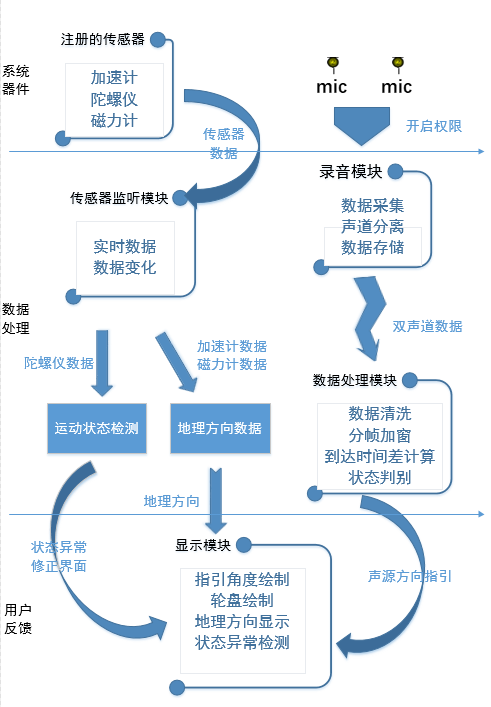
\includegraphics[width=0.8\textwidth]{dataflow.png} 
				\caption{{系统流程和数据流简图}}
				\label{fig: dataflow}
				%\vspace{0.8cm} % 用来调整和下方文字的间距
			\end{figure}
			
		\subsection{系统运行方式和界面展示}
		
			下面给出系统给出的实时指引的应用界面,具体如下图(\ref{fig: UI1},\ref{fig: UI2})所示。
			
			简要介绍应用功能,在图(\ref{fig: UI1})中,通过选择波形和对应的频率数据,点击PLAY键将可以单声道播放对应的音频,点击PAUSE即可暂停播放。
			
			\begin{figure}[H]
				\centering
				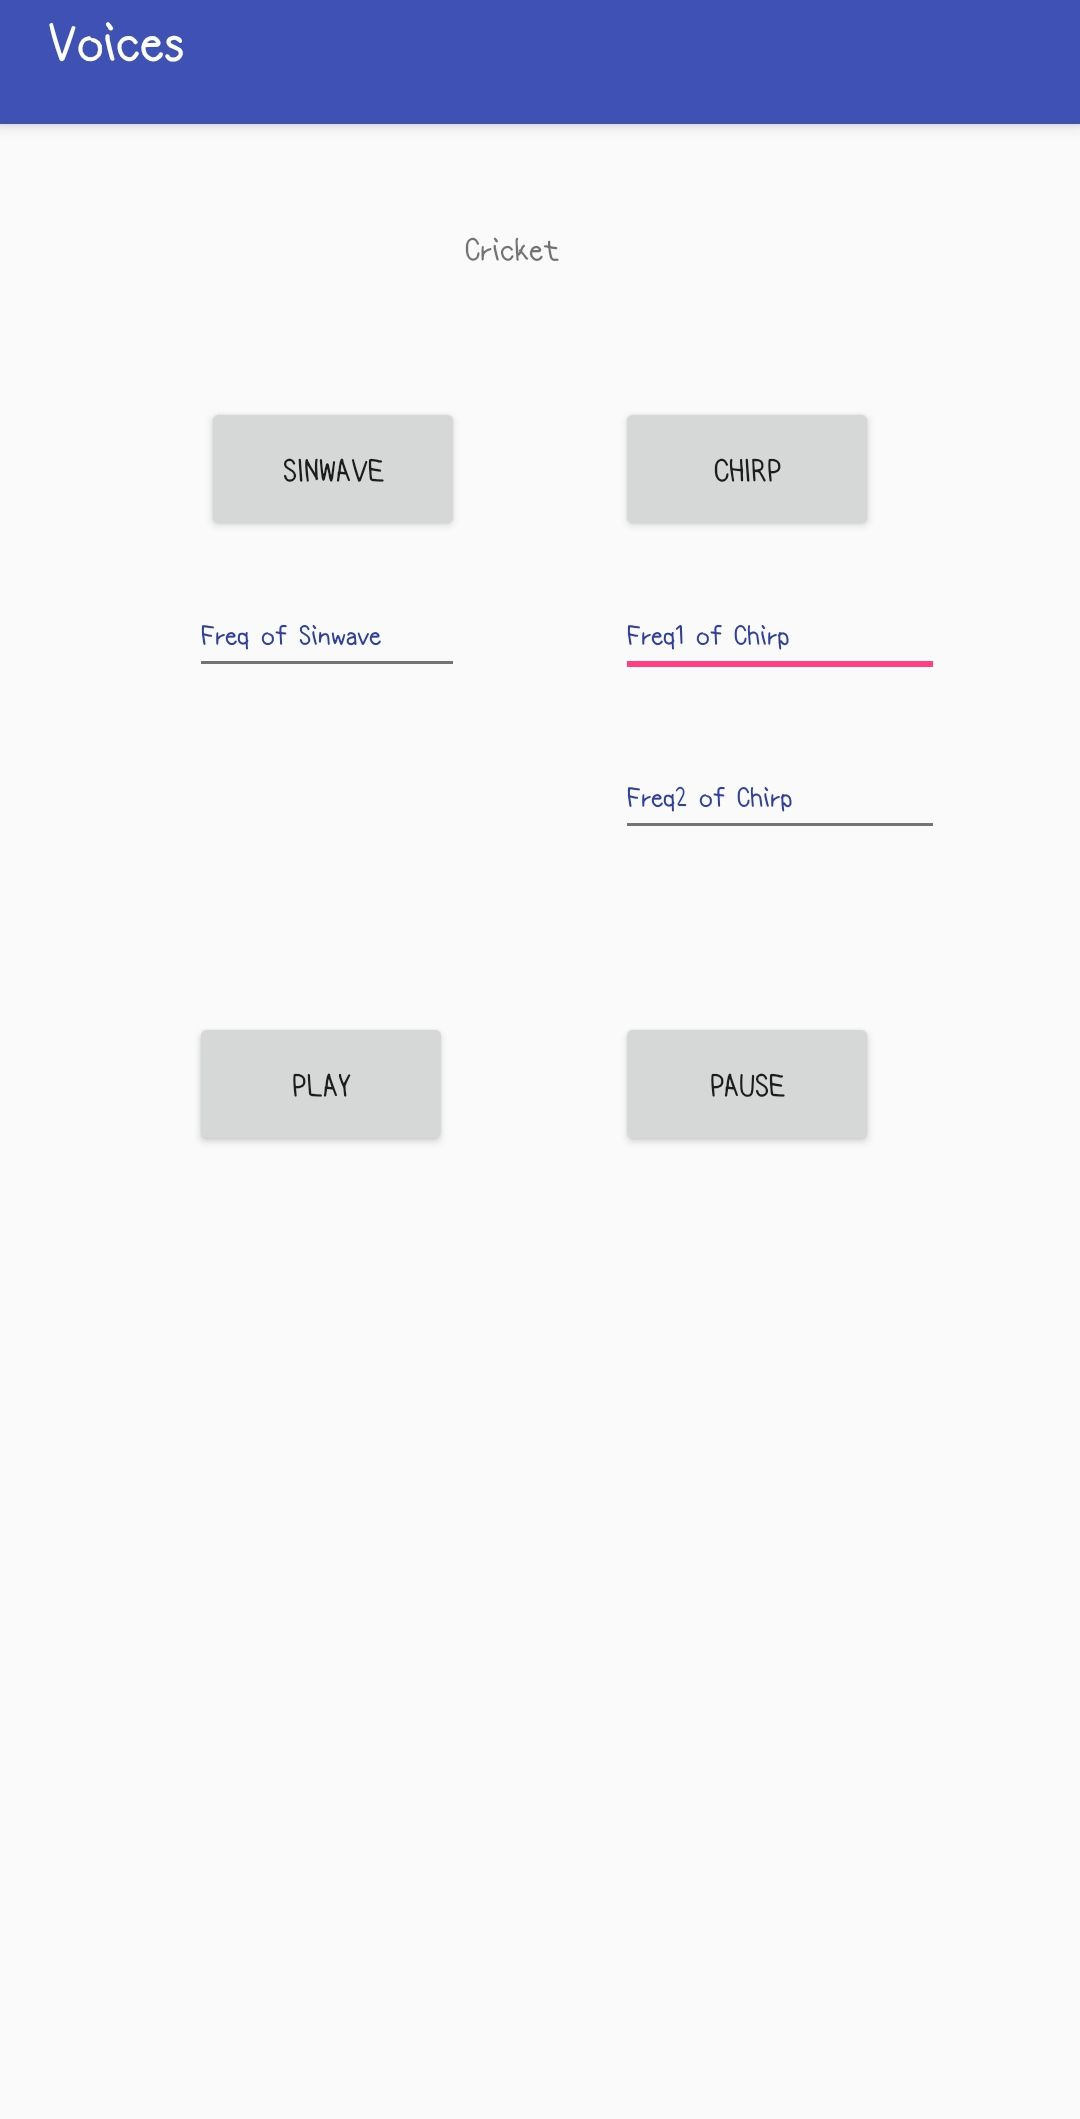
\includegraphics[width=.35\textwidth]{voice.jpg}
				\caption{发声app界面}
				\label{fig: UI1}
				%\vspace{0.8cm} % 用来调整和下方文字的间距
			\end{figure}
		
			在图(\ref{fig: UI21})中,通过选择录音,并且选择是否产生wav文件进行录音,期间可以绘制前一秒中部分的数据波形,在此界面下通过选择“产生wav文件"生成相对应的录音文件并保存在手机存储中,通过多个位置的操作,从而可以获得一系列的wav文件,这些文件将应用于后期的离线计算。
			
			在在线指引的模型下,如图(\ref{fig: UI22}),系统会默认打开麦克风并开始采集数据,当手机状态“静止时”才会收集有效数据,当产生一定量的有效数据后,系统后台将会计算出目前声源相对应手机中心的方向,也就是图中的青绿色线,并且显示与手机y轴的夹角与当前的方向(如图中“西”所示),轮盘指引的方向则是对应的地理方向,从而方便我们寻迹。
			
			
			\begin{figure}[H]
				\centering
				\begin{subfigure}{.45\textwidth}
					\centering
					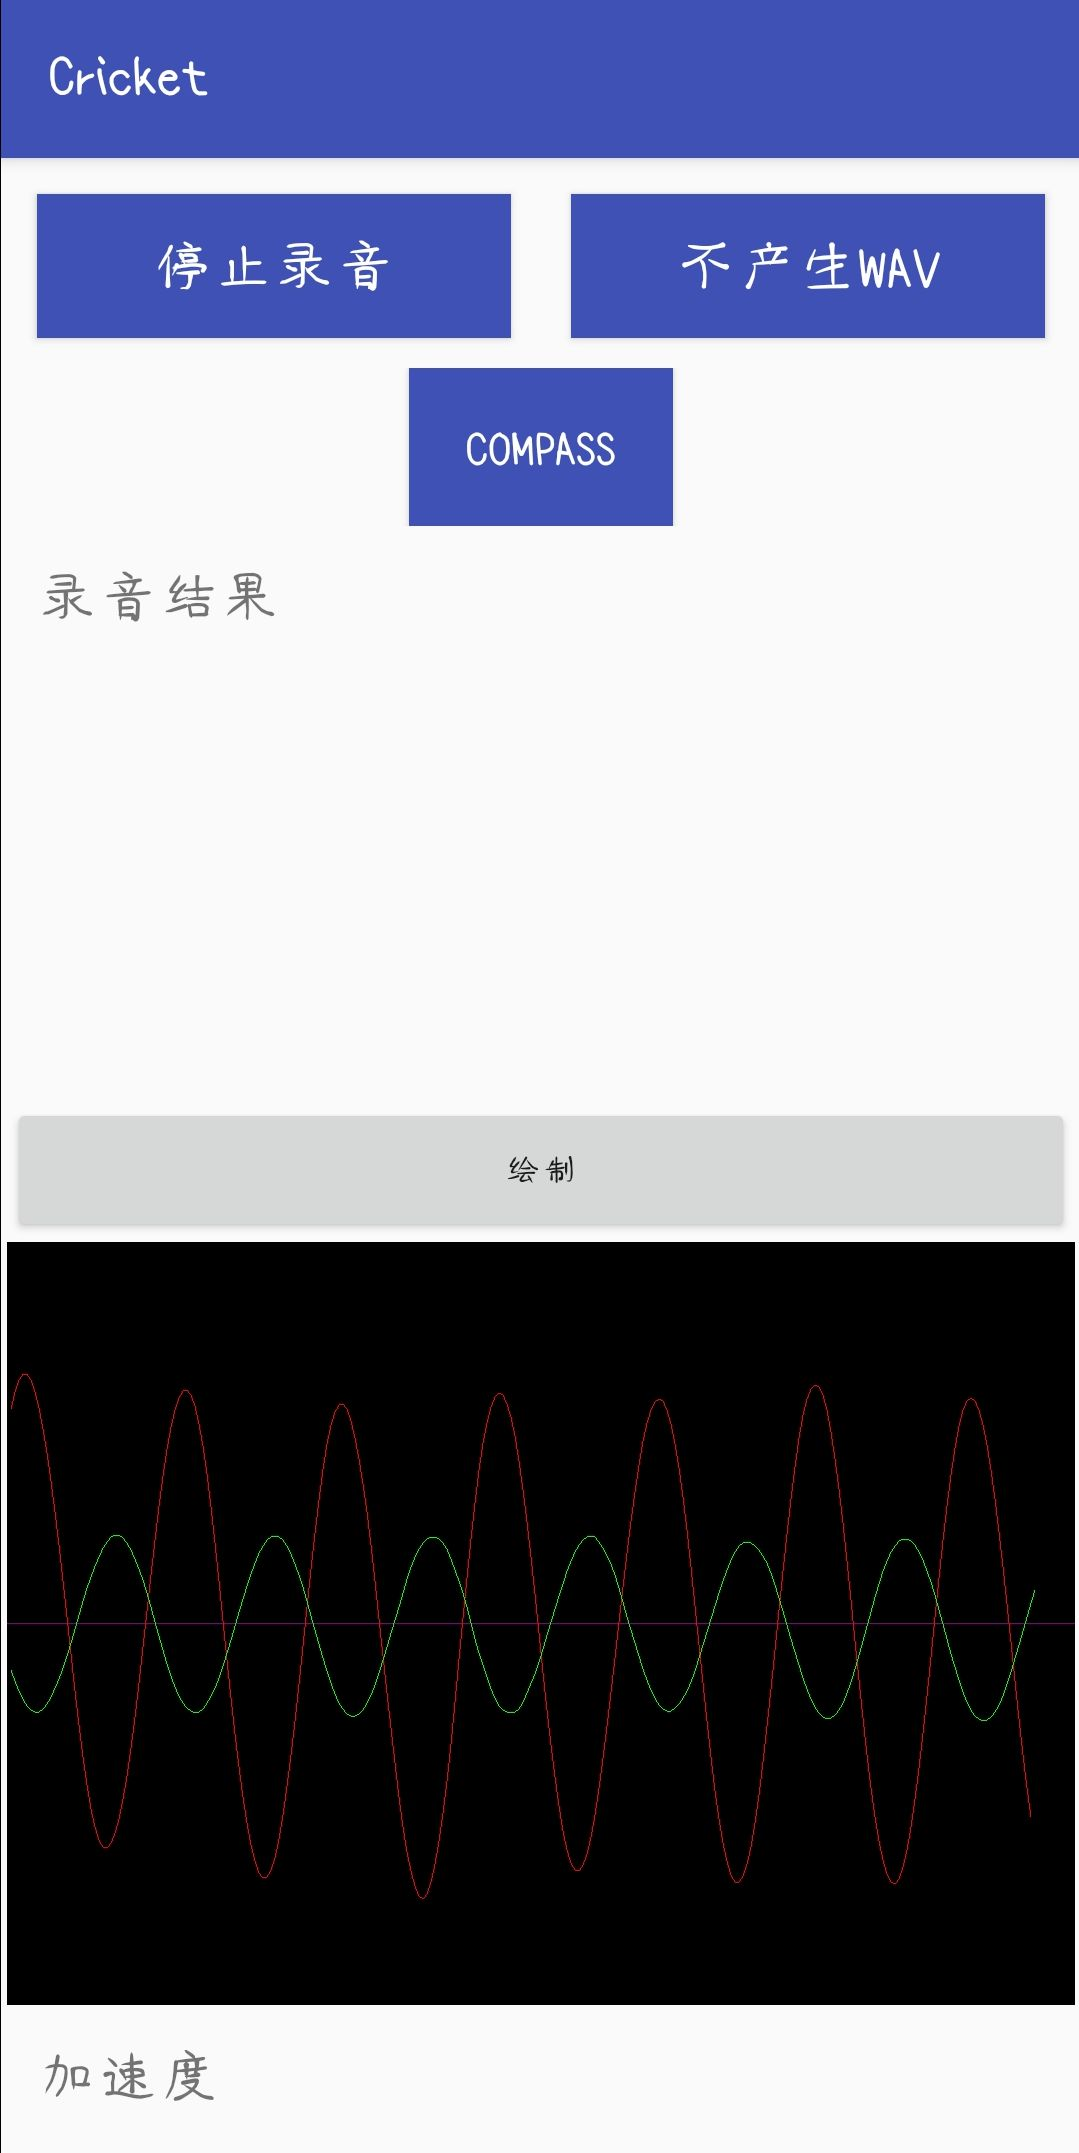
\includegraphics[width=0.6\textwidth]{collect.jpg}
					\caption{离线采集数据界面}
					\label{fig: UI21}
				\end{subfigure}
				\begin{subfigure}{.45\textwidth}
					\centering
					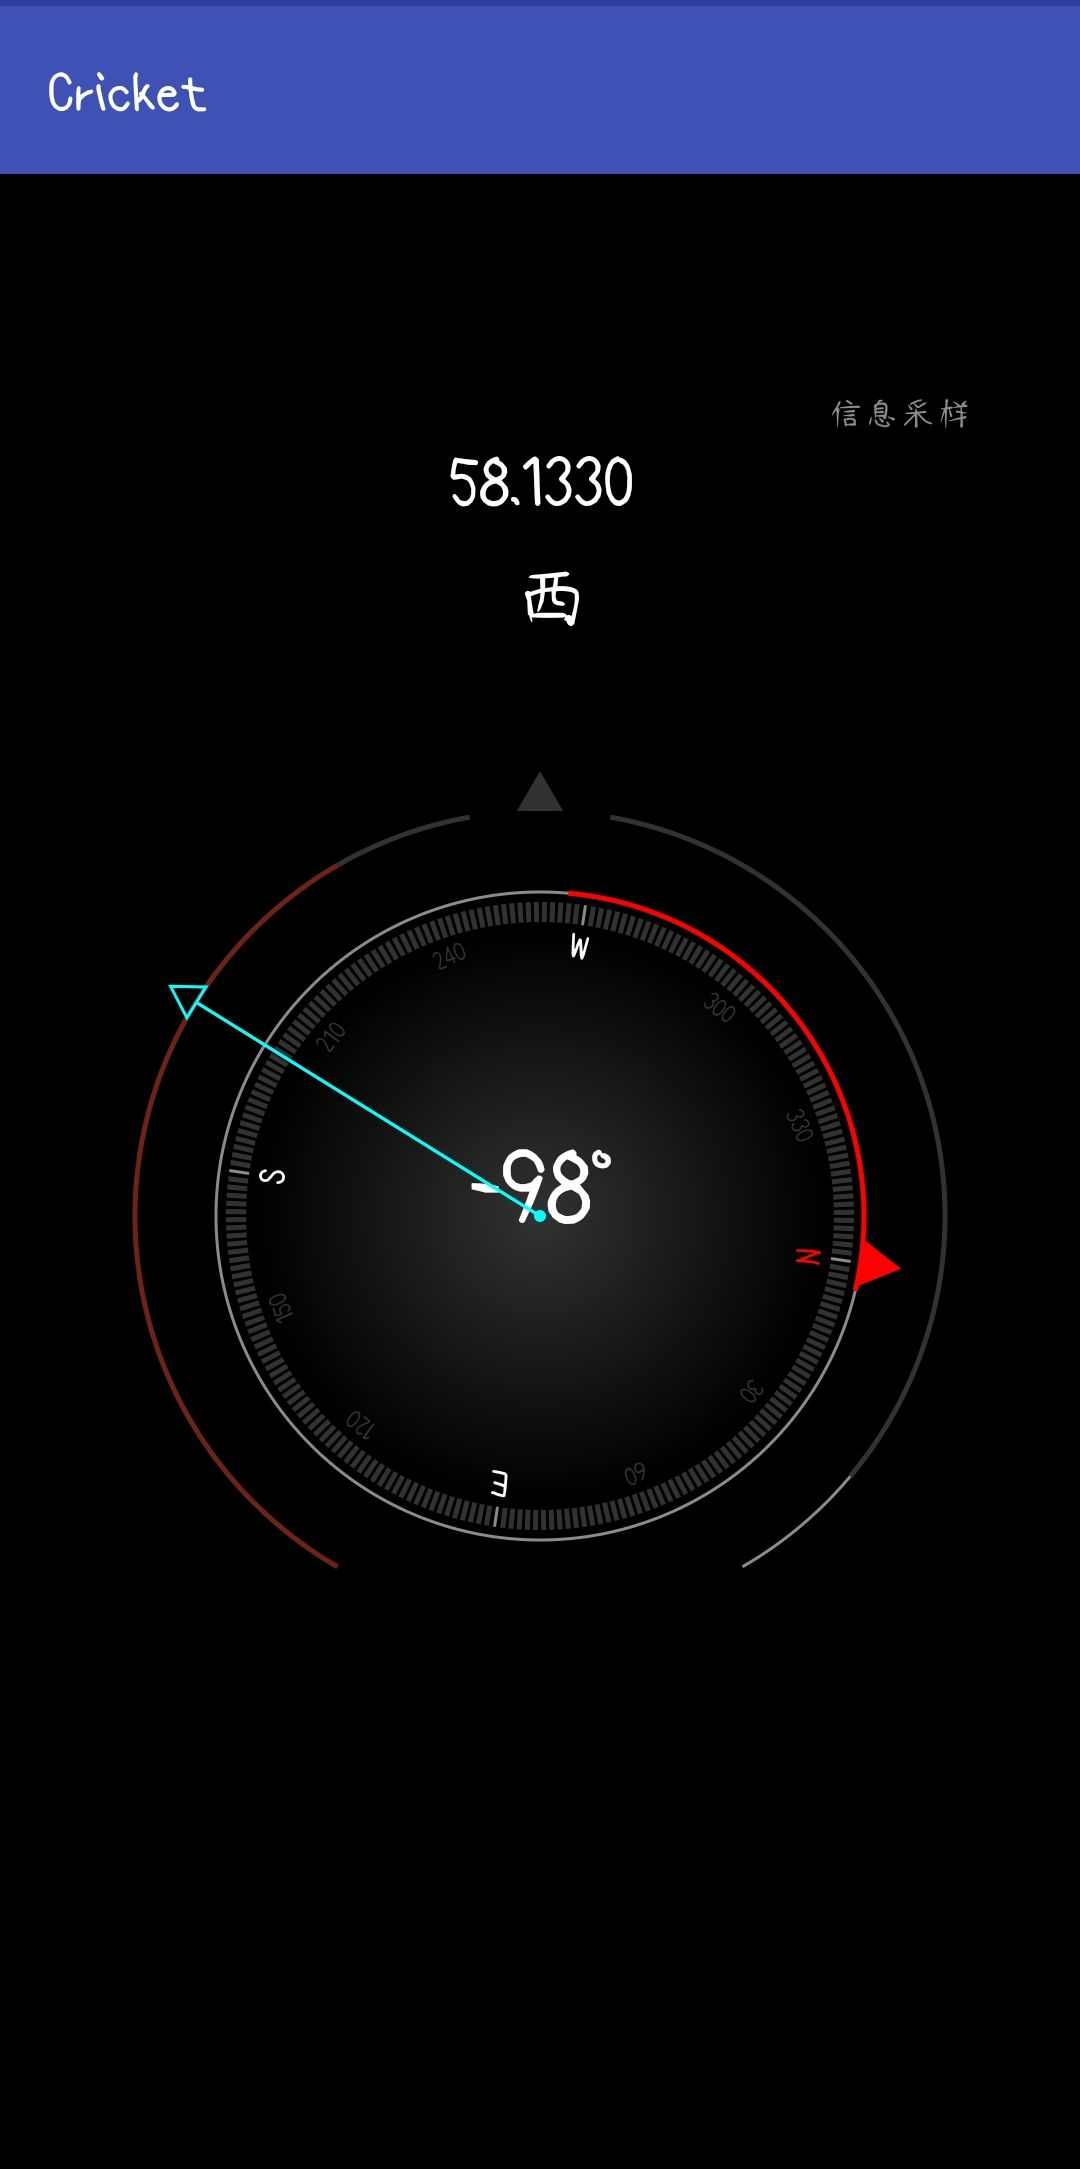
\includegraphics[width=0.6\textwidth]{compass.jpg}
					\caption{在线指引界面}
					\label{fig: UI22}
				\end{subfigure}
				\caption{(a)离线采集数据界面,(b)在线指引界面}
				\label{fig: UI2}
			\end{figure}
			
		
	\section{系统功能实现细节}
	
		\subsection{录音模块功能}
			数据采集阶段核心代码如算法\ref{alg: data-collecting}所示.手机调用双麦不断捕获周围环境中声波信号,当一个信号帧中的平均能量高于预先设定的阈值,认为可能接收到了声源信号,并且将捕获的两路声音数据进行声道分离,从而进行数据清洗等操作。
			
			\begin{breakablealgorithm}
				\caption{双麦智能手机的信号采集}
				\label{alg: data-collecting}
				\begin{algorithmic}[1]
					%\STATE {mAudioRecord.startRecording()}
					\STATE {//系统捕获环境中的音频数据} 
					\WHILE{in recording}
						\STATE {//数据帧读入音频数据} 
						\STATE {read = mAudioRecord.read(mBuffer, 0, BUFFER\_SIZE)}
						%\IF {read <= 0}
						%	\STATE {return false}
						%\ELSE
							\STATE {//硬阈值初始判断}
							\STATE { sum = accumulate()}
							\STATE {//达到设定的threshold阈值}
							\IF{sum > threshold * read}
								\STATE {两路信号分离}
								\STATE {数据转为浮点类型并存储}
								%\STATE {index = 0}
								%\FOR{$i=0$ to mBuffer.length/2}
								%	\IF{i \% 2 == 0}
								%		\STATE{System.arraycopy(mBuffer, i * 2, mBuffer1, 0, 2)}
								%		\STATE{LY[index] = ((mBuffer1[0]\&0x000000FF) | (((int)mBuffer1[1])<<8))/ 32768.0}
								%		\STATE{LYList.add(LY[index])]}
								%		\STATE{index = i / 2}
								%	\ELSE
								%		\STATE{System.arraycopy(mBuffer, i * 2, mBuffer2, 0, 2)}
								%		\STATE{RY[index] = ((mBuffer2[0]\&0x000000FF) | (((int)mBuffer2[1])<<8))/ 32768.0}
								%		\STATE{RYList.add(RY[index])]}
								%	\ENDIF
								%\ENDFOR
							\ENDIF	
							\STATE {other code for further data-processing}			
						%\ENDIF
					\ENDWHILE
				\end{algorithmic}
			\end{breakablealgorithm}
		
		\subsection{数据处理模块功能}
			
			通过麦克风采集获取的数据,将要经过滤波等清洗后并分帧进行计算。其处理流程如伪代码\ref{alg: data-handler}所示。
			
			\begin{breakablealgorithm}
				\caption{数据处理功能}
				\label{alg: data-handler}
				\begin{algorithmic}[]
					\STATE {1: 数据清洗}
						\STATE {\quad 1.1: filter(dsp)滤波}
							%\STATE {\quad \quad LSignalData = filter(bpFilt,LY)}
							%\STATE {\quad \quad RSignalData = filter(bpFilt,RY)}
							\STATE {\quad \quad [LSignalData,RSignalData] = filter(bpFilt,LY,RY)}
						\STATE {\quad 1.2: RemoveOutliers 异常点移除}
							%\STATE {\quad \quad LSD = RemoveOutliers(LSignalData,m)}
							%\STATE {\quad \quad RSD = RemoveOutliers(RSignalData,m)}
							\STATE {\quad \quad [LSD,RSD] = RemoveOutliers(LSignalData,RSignalData,m)}
					\STATE {2: 分帧加窗}	
						\STATE {\quad 2.1: [LY\_enframe,RY\_enframe] = my\_enframe(LSD,RSD, frameLen, overLoap, rect)}
						%\STATE {\quad 2.1: LY\_enframe = my\_enframe(LSD, frameLen, overLoap, 'rect')}
						%\STATE {\quad 2.2: RY\_enframe = my\_enframe(RSD, frameLen, overLoap, 'rect')}
					\STATE {3: 端点检测}
					\STATE {\quad 3.1: [VLSD,VRSD] = myVSD(LSD,RSD,Unit,m)}
						%\STATE {\quad 3.1: [VSDst,VSDed] = myVSD(LSD,RSD,Unit,m)}
						%\STATE {\quad 3.2: VLSD = LSD(VSDst:VSDed)}
						%\STATE {\quad 3.3: VRSD = RSD(VSDst:VSDed)}
					\STATE {4: 到达时间差计算}
						\STATE {\quad 4.1: 状态检测}
						\STATE {\quad 4.2: 调用自定义的Tdoa函数对两路信号进行计算}
						\STATE {\quad 4.3: [TDOA,Sign] = myTdoa(VLSD,VRSD,N,True)}
					\STATE {5: 方向角度计算与显示}
				\end{algorithmic}
			\end{breakablealgorithm}
			
		\subsection{传感器监听模块功能}
			
			通过注册和监听传感器,并实时获取传感器数据进行处理。其处理如伪代码(\ref{alg: sensor})所示。
			
			\begin{breakablealgorithm}
				\caption{传感器监听}
				\label{alg: sensor}
				\begin{algorithmic}[1]
					\STATE {//创建传感器管理器对象}
					\STATE {mSensorManager = (SensorManager)getSystemService(SENSOR\_SERVICE)}
					\STATE {//创建传感器对象}
					\STATE {mGyroscope,mAccelerometer,mMagneticField = getSensor(...)}
					%\STATE {mGyroscope = mSensorManager.getDefaultSensor(GYROSCOPE...)}
					%\STATE {mAccelerometer = mSensorManager.getDefaultSensor(ACCELEROMETER...)}
					%\STATE {mMagneticField = mSensorManager.getDefaultSensor(MAGNETIC\_FIELD...)}
					\STATE {//创建传感器监听器对象,并重写监听方法}
					\STATE {mSensorListener = new SensorEventListener()\{...\}}
					%\STATE {\quad //监听器方法重写}
					\STATE {\quad 陀螺仪数据获取}
					%\STATE {\quad gyroscopeValues = getGyroValue}
					%\STATE {\quad gyroscopeValues = event.values}
					\STATE {\quad //设备动态监测}
					\STATE {\quad IsMove(gyroscopeValues)}
					\STATE {\quad 加速计数据获取}
					%\STATE {\quad accelerometerValues = event.values}
					\STATE {\quad 磁力计数据获取}
					%\STATE {\quad magneticFieldValues = event.values}
					\STATE {//获取(计算)方向}
					%\STATE {\quad getRotationMatrix(rotation, null, accelerometerValues,magneticFieldValues)}
					\STATE {\quad getOrientation(rotation, orientation)}
					\STATE {\quad //获取方向,并更新界面}
					%\STATE {\quad chaosCompassView.changeVal(orientation[0],degree)}
					\STATE {//监听传感器}
					\STATE {registerListener(mGyroscope,mAccelerometer,mMagneticField)}
					%\STATE {mSensorManager.registerListener(mSensorListener, mGyroscope,...)}
					%\STATE {mSensorManager.registerListener(mSensorListener, mAccelerometer,...)}
					%\STATE {mSensorManager.registerListener(mSensorListener, mMagneticField,...)}
				\end{algorithmic}
			\end{breakablealgorithm}
			
		\subsection{显示模块}
		
			显示模块通过在界面已经展示,由于其实现细节主要就是对graphics库应用,与本文主要内容无关,因此在此不做描述。
		
	\section{系统性能测试和分析}
		
		对于系统的性能,下面对基于完整的双麦定位实验,以离线的定位计算模型为例,给出数据展示和分析。
		
		在离线的定位计算模型下,在前文的定位分析下,可以如图(\ref{fig: work11})所示放置智能手机和声源手机,并进行录音,其中$\text{mic}_1$为主麦,${\text{mic}_2}_k$为降噪麦依次部署的位置示意,喇叭即为声源手机放置的位置,需要说明的是,为了测量高度,因此在多次放置中,必须存在节点与其他节点不在同一平面内,如图中的${\text{mic}_2}_i$节点即表示位置高于水平面。
			
		\begin{figure}[H]
			\centering
			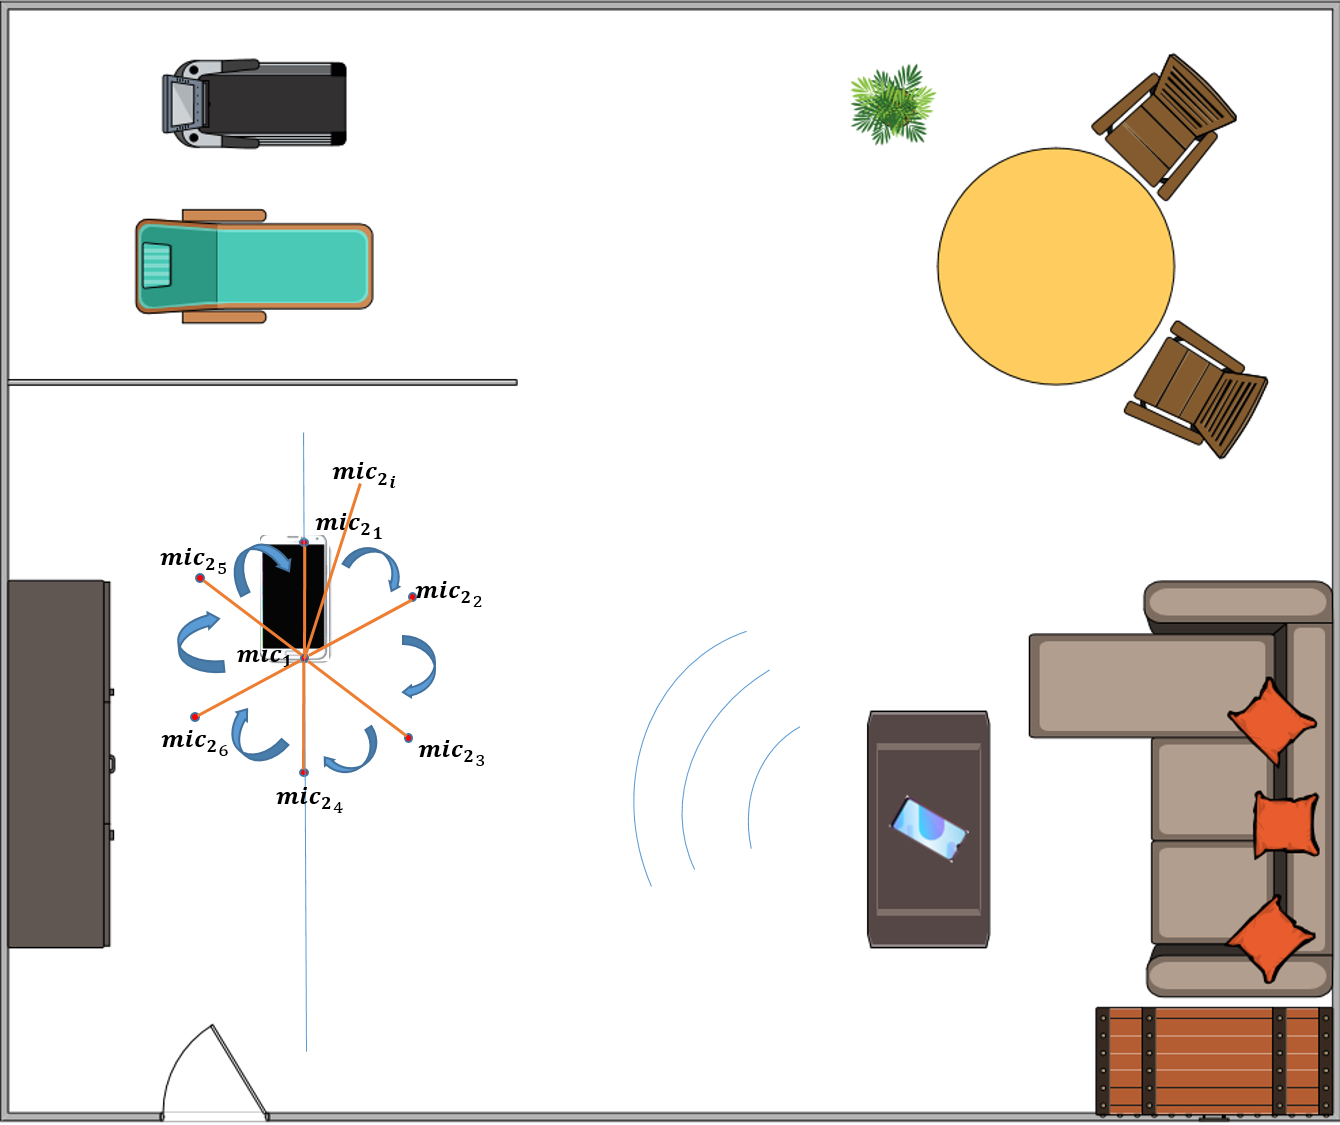
\includegraphics[width=.8\textwidth]{work11.png}
			\caption{设备放置示意}
			\label{fig: work11}
			%\vspace{0.8cm} % 用来调整和下方文字的间距
		\end{figure}
			
		随后,在三维空间下,$\text{mic}_1$为空间原点建立三轴坐标系。在室内环境下,环境非常安静,异常噪声也很少,因此数据的波动很小。通过发声手机进行周期声音的播放,并且在不同位置下进行录音。我们捕获了其中收集到一组数据,如图(\ref{fig: work12})所示。其中LY,RY代指两路麦克风收集到的信号,从中看出,尽管信号受到底层录音设备和微弱的噪声影响,会出现信号波动,但是我们仍然可以看出原始信号的周期性。利益方面,通过实际距离检测,该声源位置的空间坐标约为(200,300,117),其到达两个麦克风的距离差为8.1995cm,约为8.20cm。
			
		\begin{figure}[H]
			\centering
			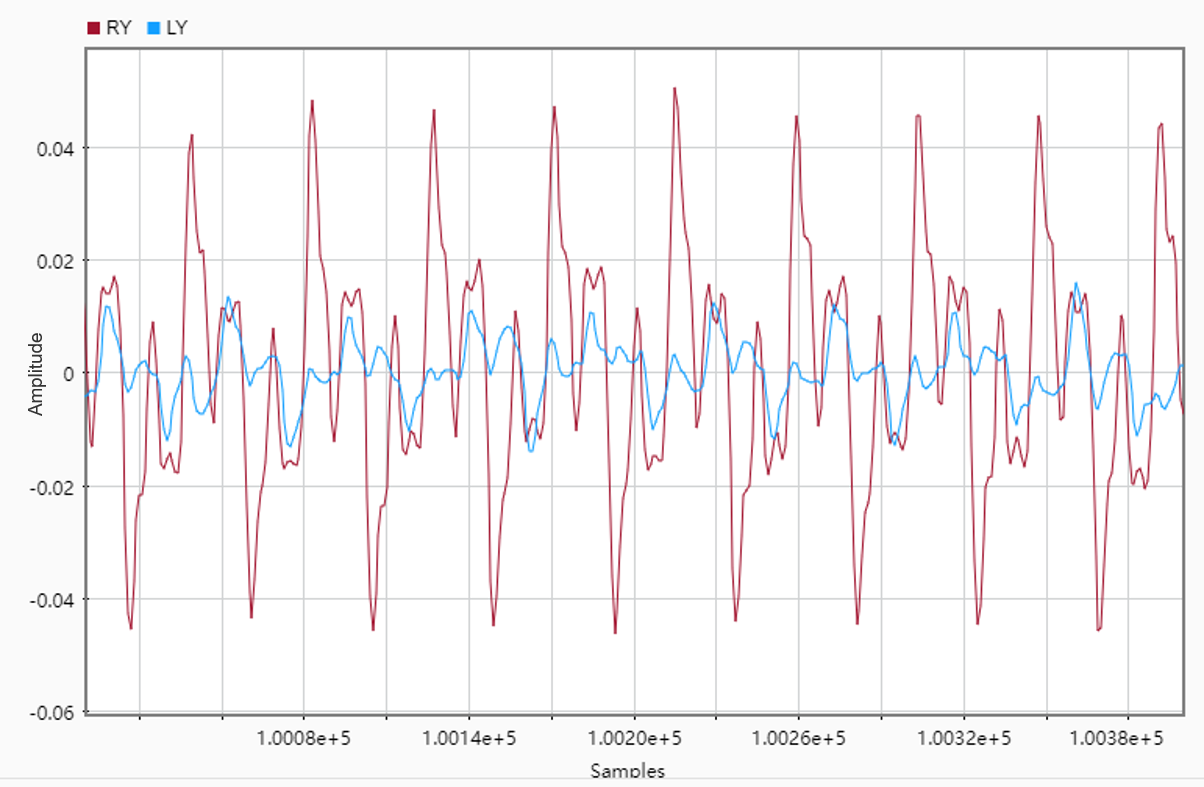
\includegraphics[width=\textwidth]{work12handled.png}
			\caption{底层原始数据部分采样}
			\label{fig: work12}
			%\vspace{0.8cm} % 用来调整和下方文字的间距
		\end{figure}
	
		根据我们在第四章的处理细节,对信号依次进行滤波加噪,异常点移除操作,对数据进行清洗,数据如图(\ref{fig: work13},\ref{fig: work14})所示。图中LSignalData,RsignalData代指经过滤波除噪后的两路信号,LSD,RSD代指异常点移除后的数据。
		
		\begin{figure}[H]
			\centering
			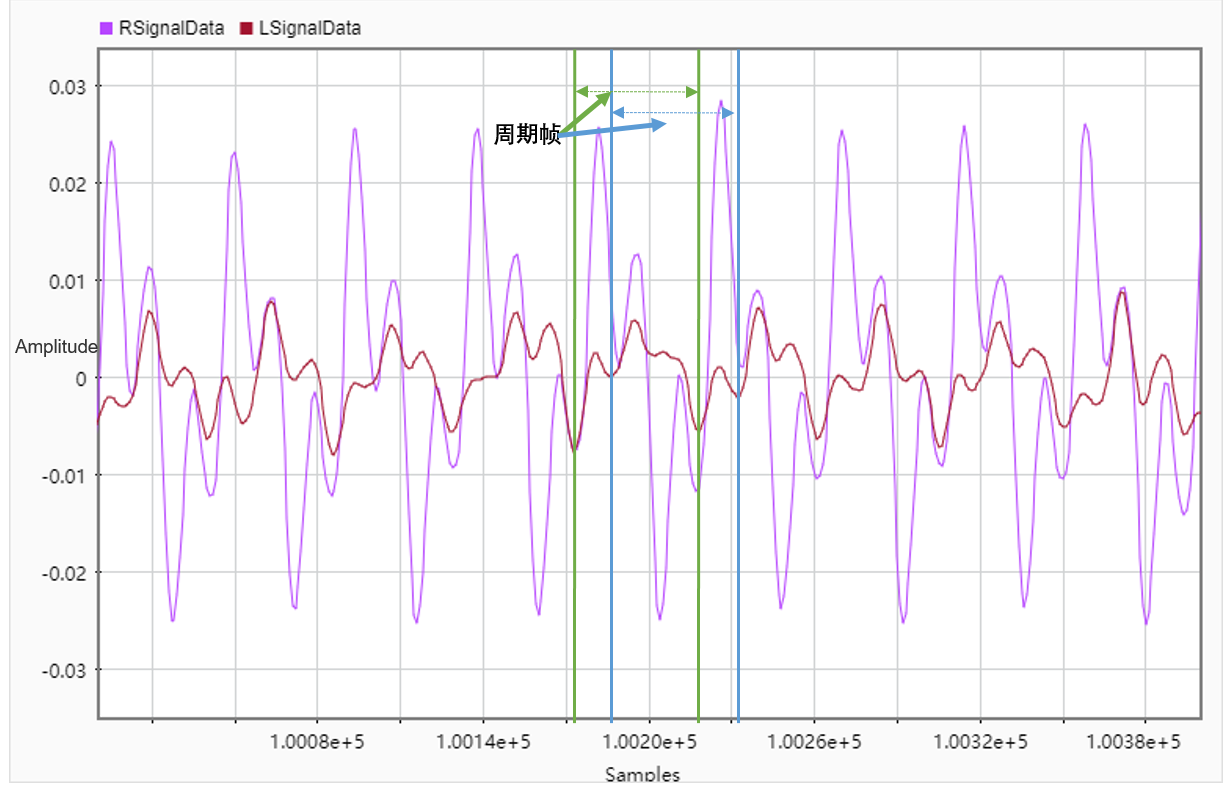
\includegraphics[width=\textwidth]{work13handled.png}
			\caption{滤波除噪后数据采样}
			\label{fig: work13}
			%\vspace{0.8cm} % 用来调整和下方文字的间距
		\end{figure}
	
	
		\begin{figure}[H]
			\centering
			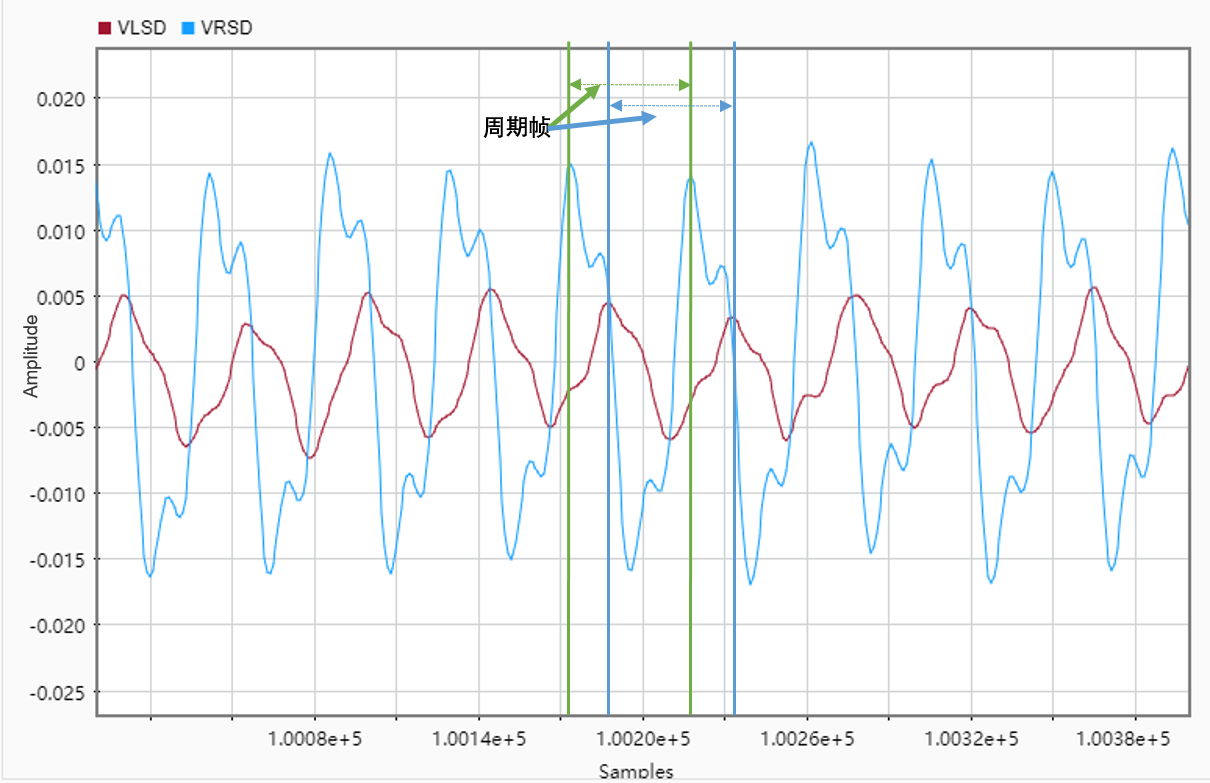
\includegraphics[width=\textwidth]{work14handled.png}
			\caption{异常点移除数据采样}
			\label{fig: work14}
			%\vspace{0.8cm} % 用来调整和下方文字的间距
		\end{figure}

		随后,对清洗后的数据进行分帧加窗等操作,最后进行到达时间差的计算。这一组数据计算的到达时间差为11个采样点,且符号正确。由于室内温度必然存在误差,前文中我们以公式(\ref{v_speed})代入计算,以室内20℃代入,则声速$v_{speed} \approx $ 343.42 m / s = 34342 cm / s,因此根据计算方案求解出的到达距离差为: $11 / 44100 * 34342 \approx 8.566$cm,与实际距离相比误差为0.366cm。
		
		最后通过matlab的计算,将多组数据进行整合计算,计算坐标为X = 198.3329cm, Y = 298.0380cm, Z = 115.3334cm,与实际坐标$X_0 $ = 200cm, $Y_0 $ = 300cm, $Z_0 $ = 117cm 相比,误差为 $\Delta X^{'}$ = 1.6671cm, $\Delta Y^{'}$ = 1.9620cm, $\Delta Z^{'}$ = 1.6666cm。
		
		综合多次测量的结果,在离线计算模型下,90\%以上计算的“左右”关系正确,到达时间差由于其必然是整数个采样点,因此很难测出准确值,但是在上面的数据我们也看出,实际误差0.366cm并没有超过一个采样点对应的距离,而70\%系统计算的到达时间点采样值误差也并不超过1个采样点,而最终计算的坐标误差,每个坐标轴的分量误差不超过10\%.
		
		
		在在线指引的模型下,以前面采集的数据为例,求解的到达距离差为8.566cm,因此,根据第四章提出的降维指引的思路,那么此阶段的指引方向角为$\arctan(\frac{8^2-4.1^2}{4.1}) = \arctan(1.6755) = 1.0327 rad = 59.1694 d$,而实际的方向在水平面投影的方向则为$\arctan(\frac{300}{192}) = \arctan(1.5625) = 1.0015 rad = 57.3817 d$,角度误差为$1.7877 d$。
		
		由于在在线指引的模型下,手机发声的功率是个很大的影响,但是由于在室内环境下,依然可以在室内较小的尺度下获得足以区分的音频强度。在大部分实验测量中,该算法都可以获得较为准确的到达时间差,尤其在3m以内的尺度下,测量的值会更准确,测量的方向角度误差在2°以内。此外,在“左右”问题的指标上,计算结果95\%以上都是正确的,因此对在线指引的及时纠正起到了很好的检测作用。	
		
		
%%%%%%%%%%%%%%%%%%%%%%%%%%%%%%%%%%%%%%%%%%%%%%%%%%%%%%%%%%%%%%%%%%%%%%%%%%%%%%%
\chapter{总结与展望}
	\section{工作总结}
		
		本文给出了关于利用具备双麦系统的智能手机实现室内定位的方案,首先对定位原理,信号时延计算原理进行阐述,又对双麦系统和智能手机及其内置传感器进行了介绍,并进而提出了离线计算和在线指引两种模型,最后在matlab和Android系统上进行了实现。本文工作涵盖了对定位方案的阐述和系统实现,以便于实验探究和后续开发。
	
	\section{前景展望}
	
		基于智能手机的应用研究会越来越深,对内置传感器的研究越来越深入,软硬件的协同发展无疑为二维空间乃至三维空间的定位和追踪带来了无限可能。除此以外,对惯性导航系统的应用也是现阶段比较热门的研究,因此将惯性系统和双麦相结合也有着广阔的发展空间。
		
		本文是一个基础性的探究性工作,虽然在室内定位方面做出了一定的贡献,但他仍然有一些不足,例如在离线定位的部署精度问题,对噪声的处理局限于室内低噪环境,在线指引的指引过程会是“离散”的指引过程,因此在这些方面都有待提高。
		
		也相信未来对智能手机双麦系统和内置传感器的研究,能够让室内定位乃至室外定位更加精确和用户友好,在这方面的研究工作也会更上一层楼。
	
	
%%%%%%%%%%%%%%%%%%%%%%%%%%%%%%%%%%%%%%%%%%%%%%%%%%%%%%%%%%%%%%%%%%%%%%%%%%%%%%%
\bibliography{sample}
%%%%%%%%%%%%%%%%%%%%%%%%%%%%%%%%%%%%%%%%%%%%%%%%%%%%%%%%%%%%%%%%%%%%%%%%%%%%%%%
	% 致谢
	\begin{acknowledgement}
		
		随着毕业论文的收笔,四年的大学生活也迎来了毕业的尾声。我依稀记得四年前拖着行李箱,来到校门口时的那份喜悦和满足,也似乎隐隐感觉到此时将要离开却无法正式告别南大的一丝落寞和酸楚。美好,充实,成长,是南大留给我的青春记忆,也是我回忆中的宝藏。
		
		在南大求学路上,遇见过很多位良师益友,他们的陪伴让我的大学生活变得充实和精彩。在学术上,他们给予我帮助和指引,也在生活中的一点一滴,带给了我属于南大的快乐记忆。
		
		首先感谢的是我的导师谢磊老师。谢磊老师不仅是一位学术上知识渊博,科研上成果丰硕的良师,更是一位生活中的益友。在本次的毕业论文中,谢磊老师不仅给了我提供了一个有趣而富有实践意义的选题思路,在实验的进展以及其他学术方面,都给了我经验之谈,让我在少走了很多弯路的同时,也让我感到了学术研究的有趣性。此外,谢磊老师让我参与到Dislab的学术团队中,让我切身感受到了科研的精彩,在两年的学习中,不断锻炼我的实践能力和表达能力,也让我的眼界和知识面都得到了拓展。谢磊老师言传身教,他的个人经历之谈,也指引着我未来的发展方向。
		
		还要感谢王楚豫博士,鲁欣然等师兄的帮助,在我初涉科研而遇很多瓶颈问题的时候,都给予了我悉心的帮助和指引,也是他们的宝贵建议,让我的实验更具有创新和挑战,也在潜移默化中锻炼我思考的能力。
		
		感谢钱柱中教授在问题求解课堂上的循循善诱,让我感受到了计算机和算法之美。感谢我的两位室友,同样作为计算机专业的学生,他们思想的火花也总是能给我带来许多灵感和创意,也非常怀念一起在深夜调试代码跑程序的“快乐”时光。
		
		最后感谢科研前辈们在本文所述的问题上作出的努力和贡献,让我能够在巨人的肩膀上看得更远。感谢戴羽彤的歌声陪伴我的日日夜夜,感谢凌晨四点的太阳,感谢科比先生,也是我一生的标杆。
		
	\end{acknowledgement}
%%%%%%%%%%%%%%%%%%%%%%%%%%%%%%%%%%%%%%%%%%%%%%%%%%%%%%%%%%%%%%%%%%%%%%%%%%%%%%%
\end{document}
